% Create a Table of Contents in Beamer
\documentclass[10pt,t]{beamer}
% Theme choice:
\usetheme{Singapore}
\useoutertheme{sidebar}
\usecolortheme{seahorse}
\setbeamercolor{titlelike}{bg=white}
\setbeamercolor{frametitle}{bg=white}
%\setbeamertemplate{frametitle}[default][left]
\setbeamertemplate{navigation symbols}{}
\setbeamertemplate{footline}{\begin{flushright}\small \insertframenumber\end{flushright}}

\usepackage{graphicx}
\usepackage{amsmath}
\usepackage{amsfonts}
\usepackage{amssymb}
\usepackage{amsthm}
\usepackage{ulem}
\usepackage{listings}
\usepackage{xcolor}
\usepackage{wrapfig}
\usepackage{subfig}
\usepackage{setspace}
\usepackage{enumerate}
\usepackage{verbatim}

% new amber color
\definecolor{amber}{rgb}{1.0, 0.75, 0.0}

% Title page details: 
\title{Chapter 3: Survival Analysis} 
\author{Nina Galanter}
\date{\today}


\begin{document}
	% Title page frame
\begin{frame}
	\titlepage 
\end{frame}

%\begin{frame}{Learning objectives}
%	By the end of Chapter 3, you should be able to:
%	
%	\begin{itemize}
%		\item Determine if a variable has been right-censored
%		\item Discuss the drawbacks of treating a right-censored variable as binary or continuous
%		\item Interpret Kaplan-Meier curves, and create them in \texttt{R}
%		\item Implement and interpret a logrank test for equating survival curves
%		\item Formulate a regression model given a scientific or statistical question about a right-censored outcome
%		\item Interpret the coefficients for a (simple or multiple) proportional hazards regression model
%		\item Interpret confidence intervals and p-values for proportional hazards regression coefficients
%		\item Use \texttt{R} to fit a proportional hazards regression model and create figures/tables to support your regression analysis
%	\end{itemize}
%	
%\end{frame}

% Outline frame
\begin{frame}{Outline}
	\tableofcontents
\end{frame}

\AtBeginSection[ ]
{
	\begin{frame}{Outline}
		\tableofcontents[currentsection]
	\end{frame}
}


\section{Characteristics of survival data}

\begin{frame}{Quantitative and binary outcomes}
Up to this point, we have focused on questions involving \textcolor{blue}{quantitative} or \textcolor{red}{binary} outcomes: 

\medskip

\begin{itemize}
\item Is \textcolor{blue}{birthweight} associated with participation in First Steps?

\medskip

\item Is \textcolor{red}{choosing to get HIV test results} associated with receiving an incentive or incentive amount? 
\end{itemize}
\end{frame}

\begin{frame}{Time-to-event outcomes}
However, we are often interested in scientific questions that involve \textcolor{blue}{time-to-event} outcomes, especially in biomedical settings:

\medskip

\begin{itemize}
\item Is time to first seizure post operation to remove a brain tumor associated with pre-operation case review by an epileptologist, in children with both epilepsy and brain tumor?

\medskip

\item Is time to promotion for university faculty members associated with gender?

\medskip

\item Is time to death from any cause associated with serum levels of C reactive protein?

\medskip

\item Is time to first COVID-19 infection associated with receiving a vaccine?

\end{itemize}
\end{frame}

\begin{frame}
\frametitle{Characteristics of survival data}
{\fontsize{9pt}{7.2}\selectfont
Sample of the observed times until first severe panic attack (in weeks):

\medskip

\begin{tabular}{|c|c|c|c|c|c|c|c|c|c|}
\hline
\textcolor{blue}{meditation} & 14.29 & 7.74 & 21 & 25.18 & 2.83 & 17.57 & 19.13 & 0.14  \\
\hline
placebo & 21 & 3.94 & 7.77 & 6.54 & 24 & 12.55 & 21.29 & 3.58 \\
\hline
\end{tabular}
}

We wish to study whether \textcolor{blue}{meditation} prolongs the \textcolor{purple}{time until a severe panic attack} in patients suffering from a panic disorder. We:

\medskip

\begin{enumerate}
\item recruit 200 patients and randomize them to meditation or placebo;

\medskip

\item follow each patient until their first severe panic attack post-recruitment;

\medskip

\item use a t-test to compare the mean time until a severe panic attack in each group
\end{enumerate}
\vfill

	Note that these data are simulated!

\end{frame}

\begin{frame}
\frametitle{Characteristics of survival data}
\centering
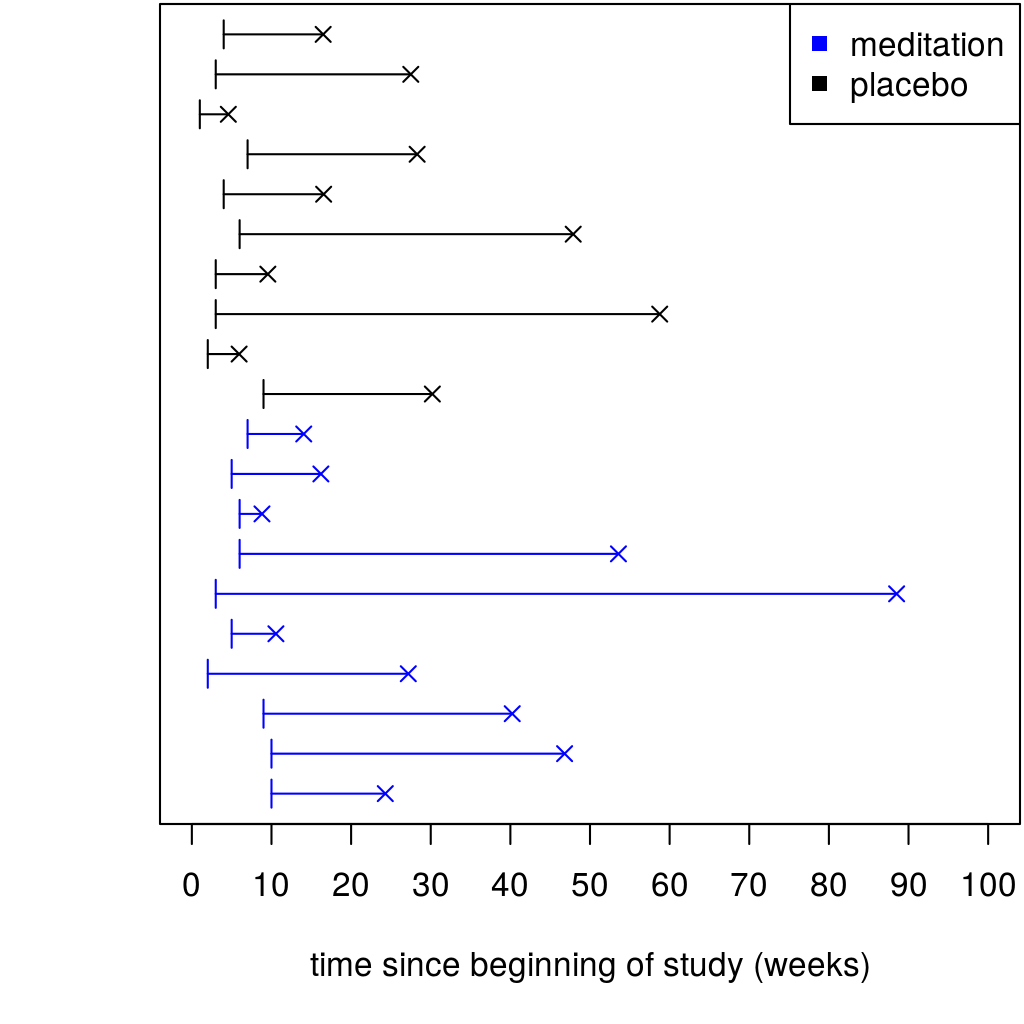
\includegraphics[width=0.7\textwidth]{figs/meditation_observed_study_time.png}
\end{frame}

\begin{frame}
\frametitle{Characteristics of survival data}
\vspace{-0.8cm}
We don't care about time from the beginning of the study until a panic attack, but rather the \textcolor{blue}{time from when the patient was randomized} to meditation/placebo
\begin{center}
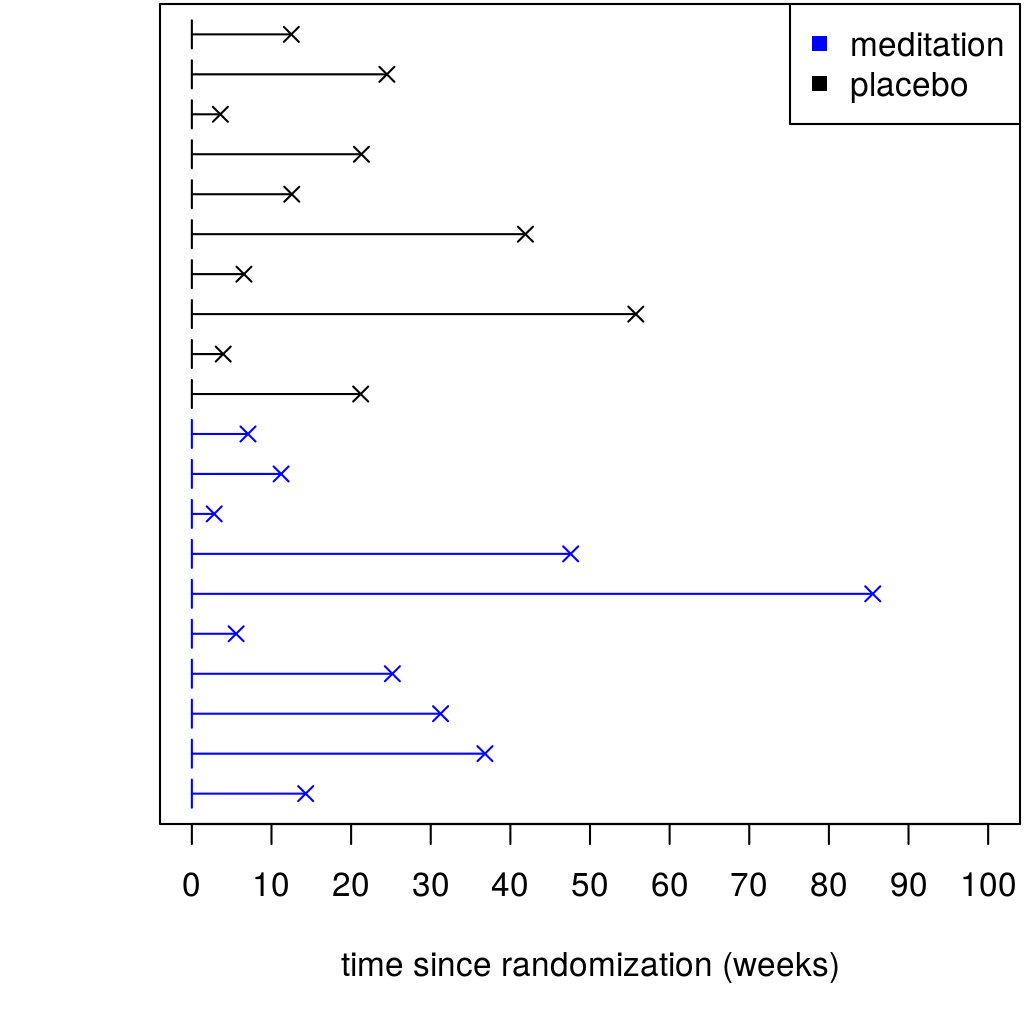
\includegraphics[width=0.7\textwidth]{figs/meditation_observed_rand_time.png}
\end{center}
\end{frame}

\begin{frame}
\frametitle{Characteristics of survival data}

\vspace{-5 mm}

In this hypothetical study, we were able to record the actual time of panic attack \textcolor{blue}{for each participant}.
\\ ~\ 

Is this typical of human studies?   \textcolor{red}{No!}
\\ ~\ 

Why?   Some common reasons are:
\medskip

\begin{itemize}
\item the study ended (e.g., after 30 weeks) and some participants had not yet had a severe panic attack (\textcolor{blue}{administrative censoring})

\smallskip

\item the participant left the study before having had a severe panic attack (\textcolor{blue}{loss to follow-up})
\end{itemize}
\medskip

If we're watching people and waiting for some health-related event to occur, it's not realistic for us to observe that event for everyone in our study. 
\\ ~\ 

This leads to \textcolor{blue}{\textbf{right-censored}} data, where rather than knowing the event time exactly, we know that it exceeds some cutoff.
\end{frame}

\begin{frame}
\frametitle{Characteristics of survival data}
\vspace{-0.8cm}
Suppose that we only have resources to run the study for \textbf{30 weeks}, and some people also stop returning to the clinic for follow-up visits. We indicate the last time we saw a patient using a circle.  
\begin{center}
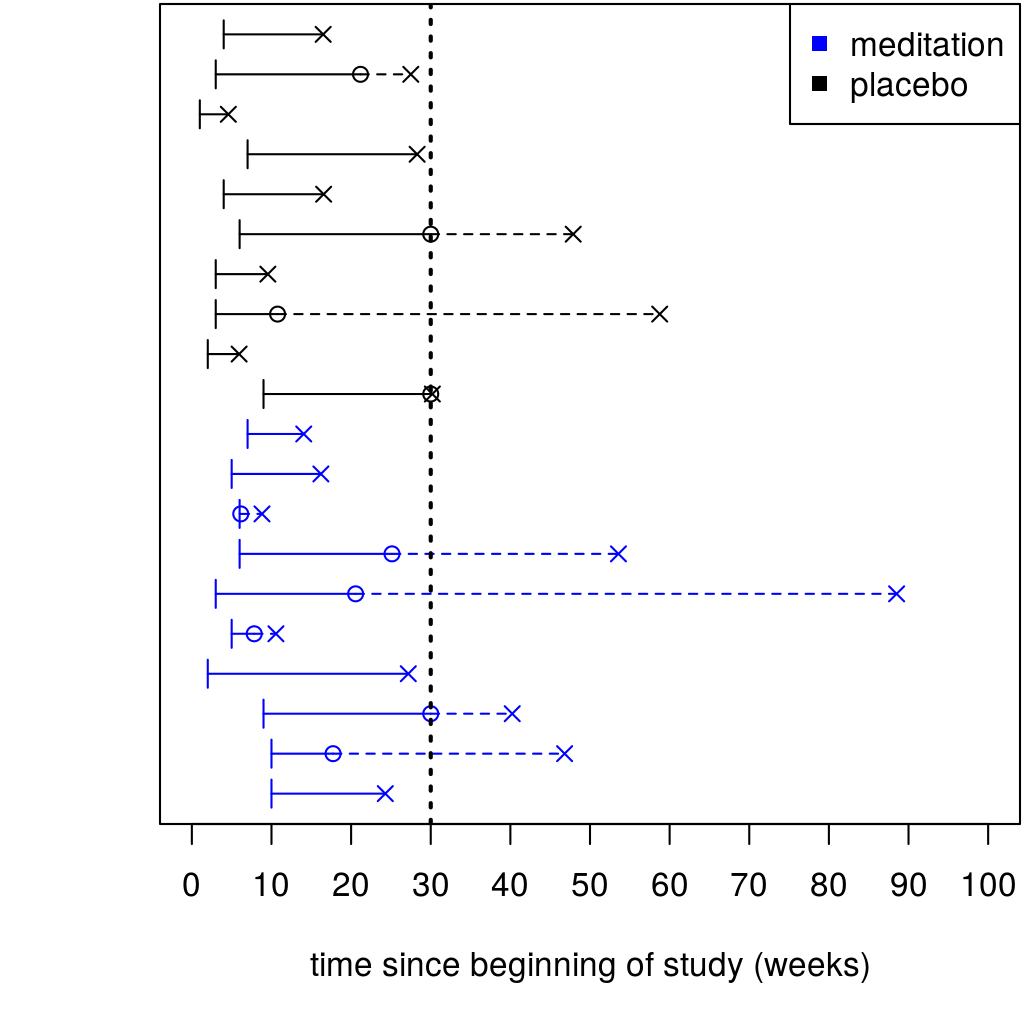
\includegraphics[width=0.7\textwidth]{figs/meditation_censored_study_time.png}
\end{center}
\end{frame}

\begin{frame}
\frametitle{Characteristics of survival data}
\centering
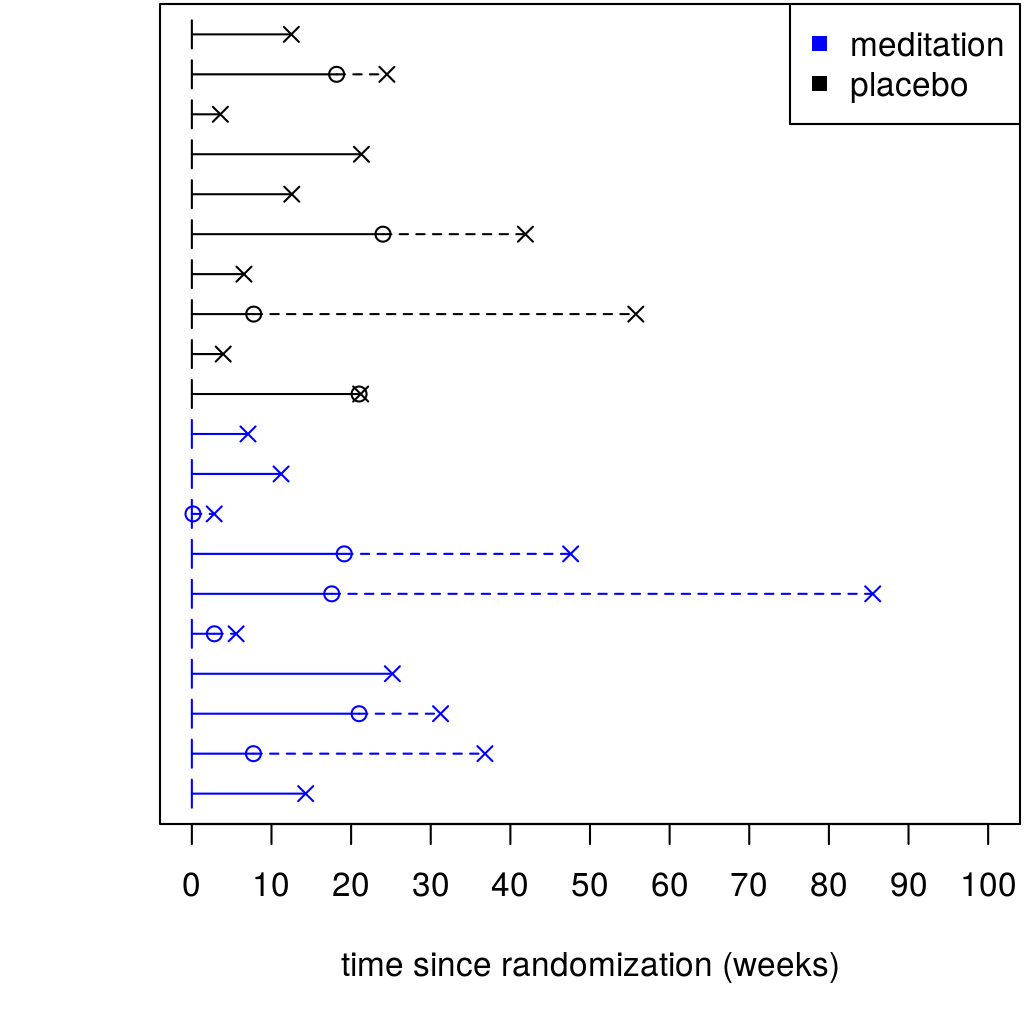
\includegraphics[width=0.7\textwidth]{figs/meditation_censored_rand_time.png}
\end{frame}

\begin{frame}
\frametitle{Characteristics of survival data}

\vspace{-6 mm}
The data can be represented as:
\medskip

{\fontsize{7.5pt}{7.2}\selectfont
\begin{tabular}{|c|c|c|c|c|c|c|c|c|c|}
\hline
\textcolor{blue}{meditation} & 14.29  & \textcolor{red}{7.74+} & \textcolor{red}{21.00+} & 25.18  &  \textcolor{red}{2.83+} & \textcolor{red}{17.57+} & \textcolor{red}{19.13+} &  \textcolor{red}{0.14+}  \\
\hline
placebo & \textcolor{red}{21.00+} &  \textcolor{red}{3.94+} &  \textcolor{red}{7.77+} &  6.54  & \textcolor{red}{24.00+} & 12.55  & 21.29 &  3.58 \\
\hline
\end{tabular}
}

Should we throw out these incompletely observed times?   

\smallskip

 \textcolor{red}{No!! This is a bad idea because:} 

\medskip

\begin{itemize}
\item Censored observations contain valuable information:  

\medskip
\begin{itemize}
\item \textcolor{red}{20+}: the participant did not experience a severe panic attack before 20 weeks  

\medskip

	\item their actual time until the first severe panic attack must be in the interval $(20, +\infty)$ 

\end{itemize}
\medskip

\item Uncensored observations are \textbf{not representative of the whole study population}

\begin{itemize}
	\medskip
	
	\item valid estimation and inference when excluding missing data (which we have done so far in this course) assumes those excluded are ``similar to'' those still in the data (\textbf{missing completely at random})
\end{itemize}
  
\end{itemize}

\end{frame}

\begin{frame}
\frametitle{Missing data}
Think about the following questions:

\medskip

\begin{enumerate}
\item Are those with smaller or larger times more likely to be censored? Why?  

\medskip

\item Systematically excluding censored times could lead to \textcolor{red}{biased estimates}. Would this lead to an overestimation or an underestimation of the \textcolor{blue}{mean} time until severe panic attack? Why?
\end{enumerate}

\end{frame}

\begin{frame}
\frametitle{Missing data}

\vspace{-5 mm}

\begin{enumerate}
\item Are those with smaller or larger times more likely to be censored? 
\medskip

\item[] \textcolor{blue}{Those with \textbf{larger times} are more likely to be censored; we only get to observe these people for a comparatively small amount of time, so we may miss their event. For example, people with time from randomization to first panic attack of more than 30 weeks are guaranteed to be censored.}  

\medskip

\item Systematically excluding censored times could lead to \textcolor{red}{biased estimates}. Would this lead to an overestimation or an underestimation of the mean time until severe panic attack?

\medskip

\item[] \textcolor{blue}{\textbf{Underestimation}: if we exclude censored times, then we are effectively excluding these people with potentially longer times, and losing all of this information!}
\end{enumerate}

\end{frame}

\begin{frame}
\frametitle{Missing data}

\vspace{-7 mm}

Distribution of times in participants who become censored or uncensored, and the overall target population:
\begin{center}
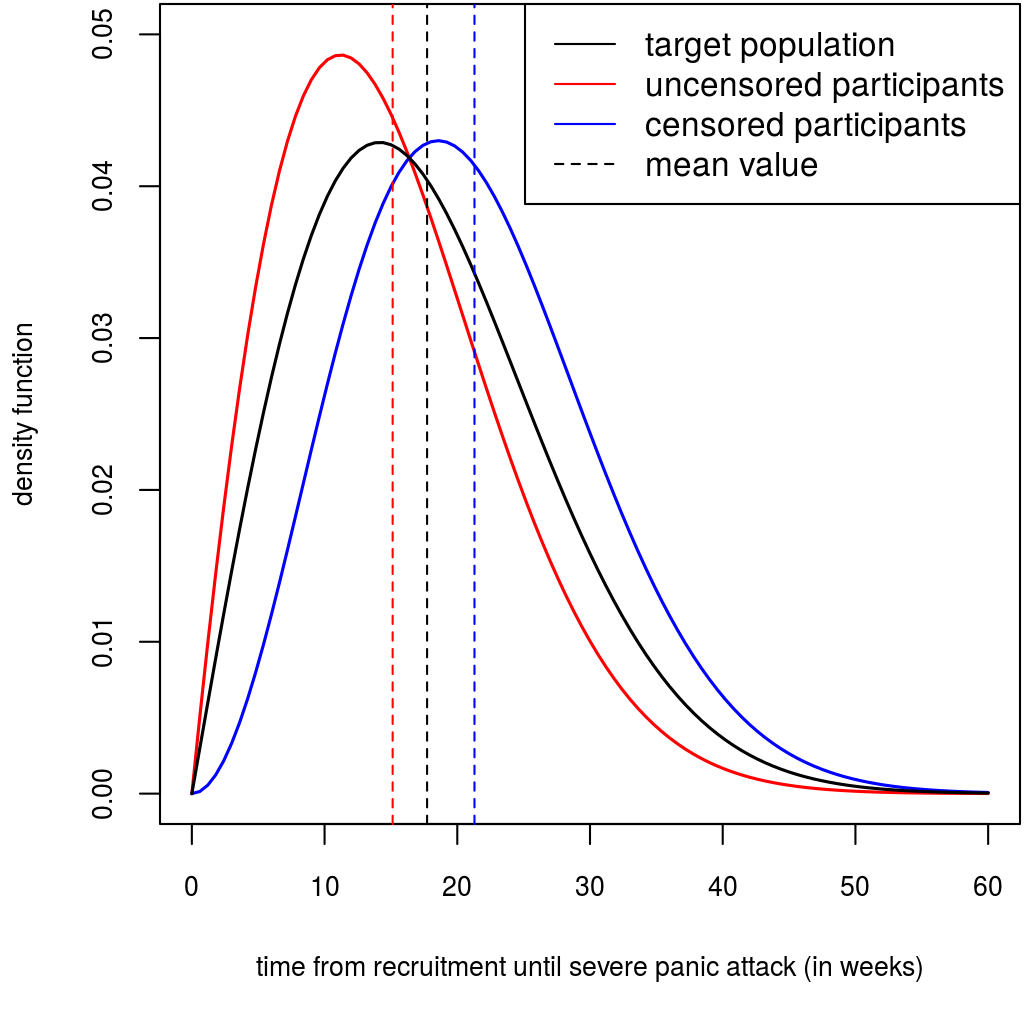
\includegraphics[height=\textheight]{figs/meditation_density_versus_obs_time.png}
\end{center}
\end{frame}

\begin{frame}
\frametitle{Survival analysis}
\textcolor{blue}{\textbf{Survival analysis}} is the branch of statistics concerned with the analysis of \textcolor{blue}{\textbf{time-to-event data}}.

\vspace{0.3cm}

Often, the goals of a survival analysis are to:
\medskip

\begin{itemize}
\item describe the distribution of a time-to-event variable

\medskip

\item compare the time-to-event distribution in different subpopulations

\medskip

\item investigate the relationship between explanatory variables and the time-to-event distribution
\end{itemize}

\vspace{0.3cm}

Even when our time-to-event data do not truly mean survival (e.g., time to first severe panic attack), we still use the term ``survival". 
\end{frame}

\begin{frame}
\frametitle{Characteristics of survival data}

\vspace{-7 mm}

Why makes time-to-event data special? Why not use standard methods? 
\medskip

\begin{itemize}
\item A time-to-event variable is always positive and generally skewed  
\medskip

\item To appropriately define a time-to-event, we must specify:  
\medskip

\begin{itemize}
\item \textcolor{blue}{initiating event} --- e.g., birth, recruitment into study, onset of disease   

\medskip

\item \textcolor{blue}{terminating event} --- e.g., death, onset of disease 
\medskip
 
\item \textcolor{blue}{time scale} --- e.g., calendar time, number of transfusions  
\end{itemize}
\medskip

\item Time-to-event data are generally observed subject to some incompleteness, of which \textbf{censoring} is a major type. Throwing away incomplete data generally results in
\medskip

\begin{enumerate}
\item a loss of information (and increase in estimation uncertainty)

\medskip
\item \textbf{\textcolor{blue}{biased estimation procedures (most important!)}}
\end{enumerate}

\end{itemize}

\end{frame}

\begin{frame}
\frametitle{Other types of censoring}
A variable is \textcolor{blue}{\textbf{censored}} if rather than being known exactly, it is known to lie in some set of values.
\\ ~\ 

In this course, we will focus on \textcolor{blue}{\textbf{right censoring}}, where we only know that the event occurred after the censoring time. This is what we've seen so far. 
\\ ~\ 

Right-censored data are the most common type of censored data found in applications! But you could also have 

\medskip
 
\begin{itemize}
	\item Left censoring: We only know the event occurred before the censoring time  
	
	\medskip
	
	\item Interval censoring: We only know the event happened between two times, but don't know exactly when
\end{itemize}
\end{frame}

% risk set, plus movie
\begin{frame}
\frametitle{Risk set}

\vspace{-5 mm}

A key concept in survival analysis is the \textbf{risk set}.
\\ ~\ 

\textbf{Risk set at time $t$}: the collection of participants that \textcolor{blue}{could have experienced} the event at time $t$; in other words, those who were still at-risk at time $t$. We denote this \textcolor{blue}{$R(t)$}. 
%\begin{align*}
%\textbf{fraction at risk at time } t = & \frac{\textbf{size of risk set at time } t}{\textbf{total sample size}}.
%\end{align*}
\bigskip

A few observations:
\medskip

\begin{itemize}
\item participants \textcolor{blue}{exit} the risk set either when they \textcolor{blue}{experience an event} or when they \textcolor{red}{become right-censored}

\medskip

\item with right-censored data, all participants are in the risk set at time 0 and the risk set necessarily shrinks over time

\medskip

\item the \textcolor{blue}{size of the risk set} and the \textcolor{blue}{characteristics of its members} will be critical in survival analysis
\end{itemize}
\end{frame}

\begin{frame}
\frametitle{Risk set}
\begin{center}
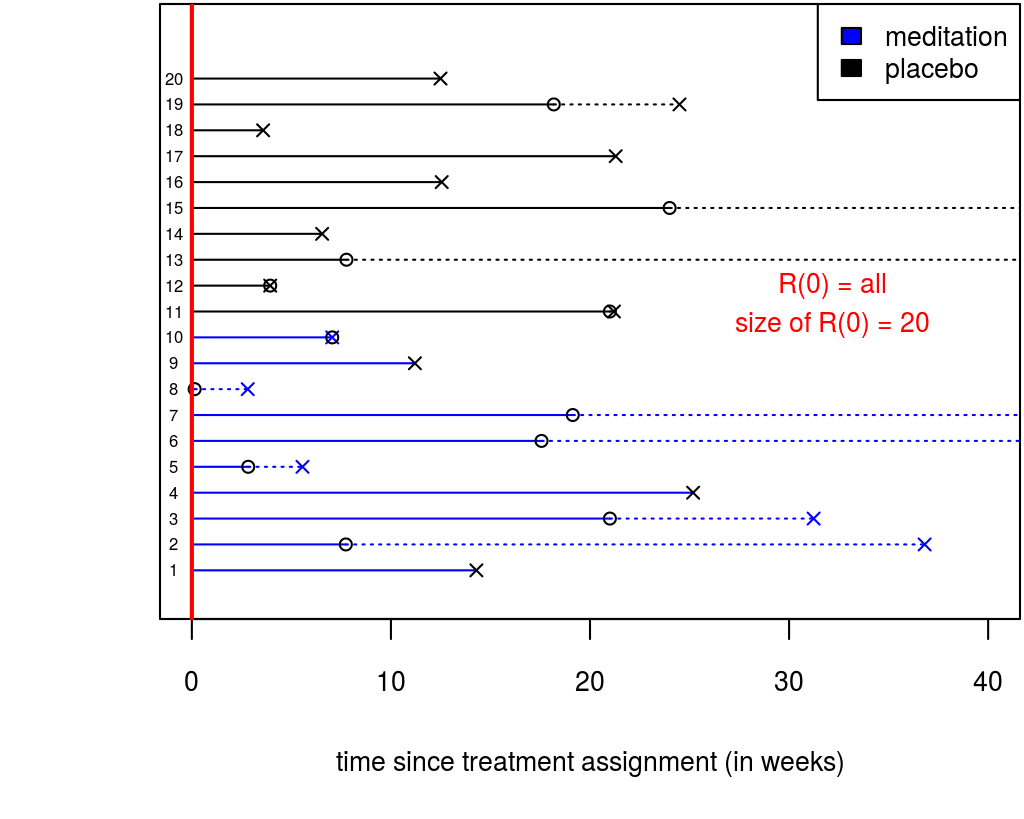
\includegraphics[height=0.8\textheight]{figs/risk_set_movie_0.png}
\end{center}
\end{frame}

\begin{frame}
\frametitle{Risk set}
\begin{center}
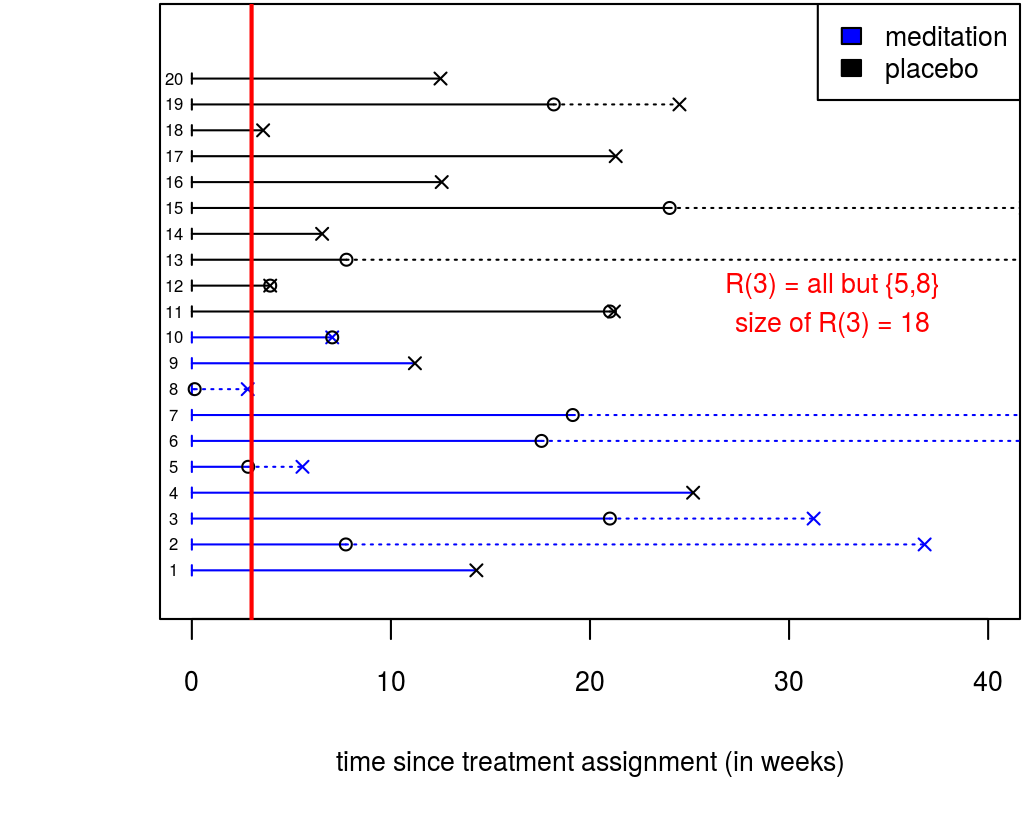
\includegraphics[height=0.8\textheight]{figs/risk_set_movie_1.png}
\end{center}
\end{frame}

\begin{frame}
\frametitle{Risk set}
\begin{center}
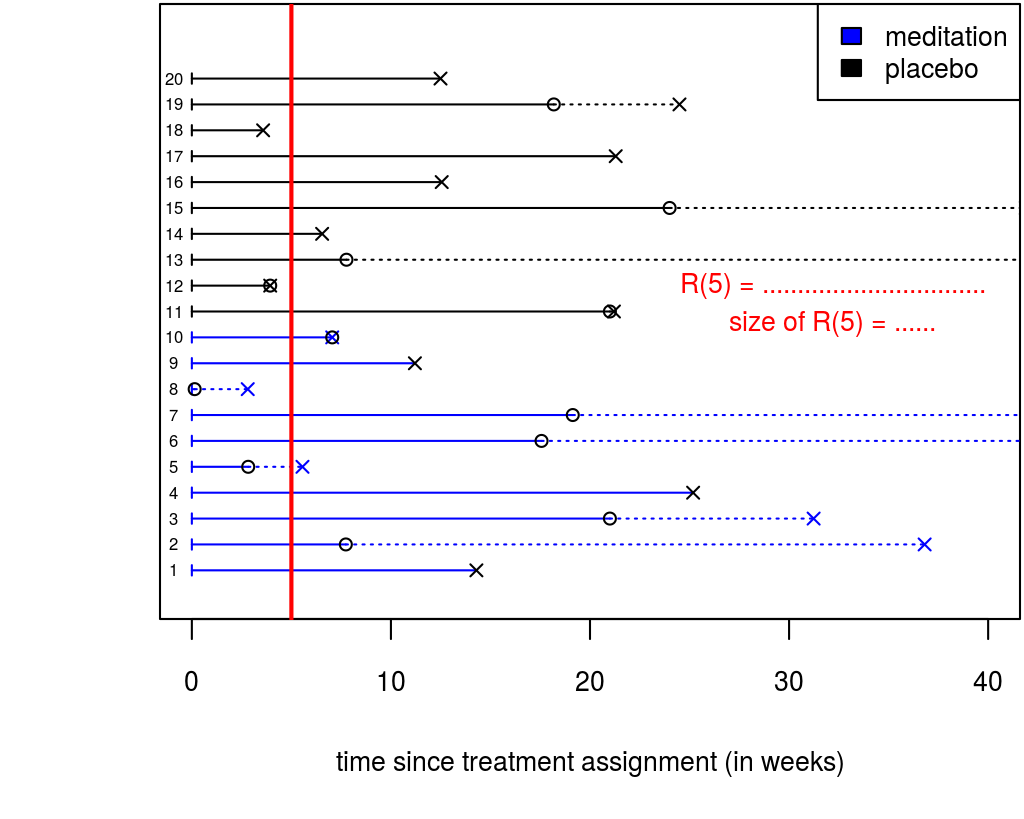
\includegraphics[height=0.8\textheight]{figs/risk_set_movie_2.png}
\end{center}

\textcolor{violet}{Pollev: \href{https://PollEv.com/free_text_polls/7351VWJoQzih5iGOeImh2/respond}{link}} What is the size of the risk set at 5 weeks? \pause\textcolor{blue}{16}


\end{frame}

\begin{frame}
\frametitle{Risk set}
\begin{center}
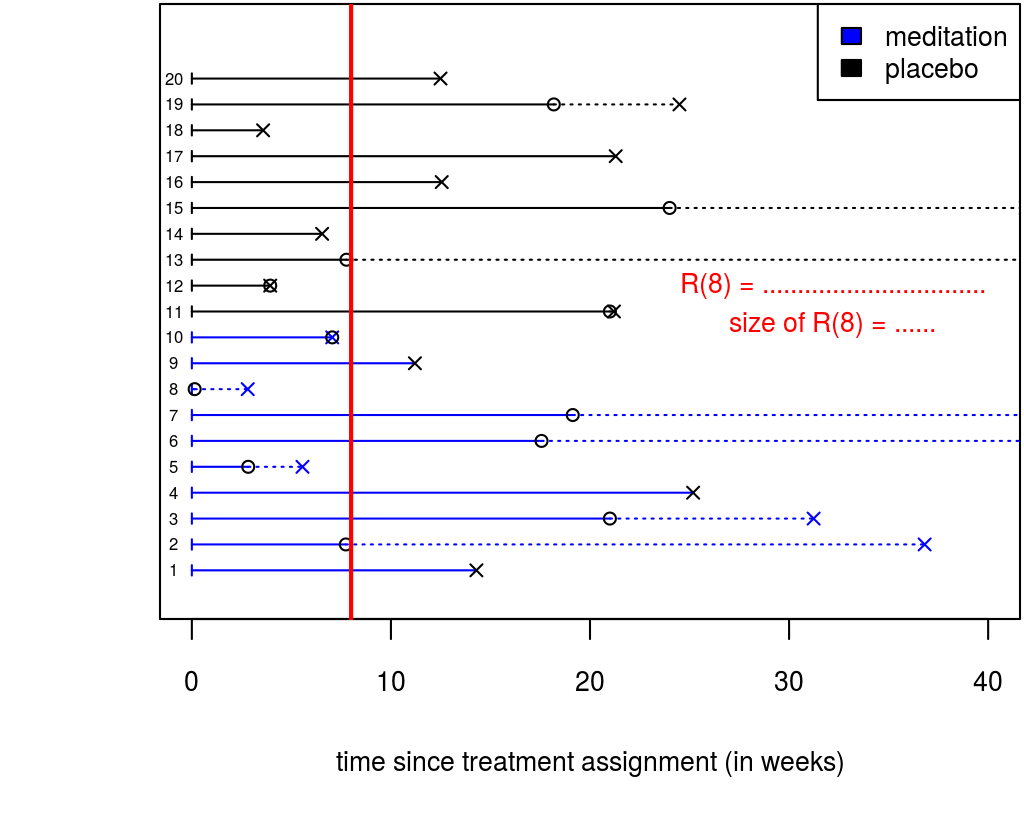
\includegraphics[height=0.8\textheight]{figs/risk_set_movie_3.png}
\end{center}

\textcolor{violet}{Pollev: \href{https://PollEv.com/free_text_polls/5lZONvVj6OxOmvX0N1BHP/respond}{link}} What is the size of the risk set at 8 weeks? (include people who were censored at 8 weeks) \pause\textcolor{blue}{14}



\end{frame}

\begin{frame}
\frametitle{Risk set}
\begin{center}
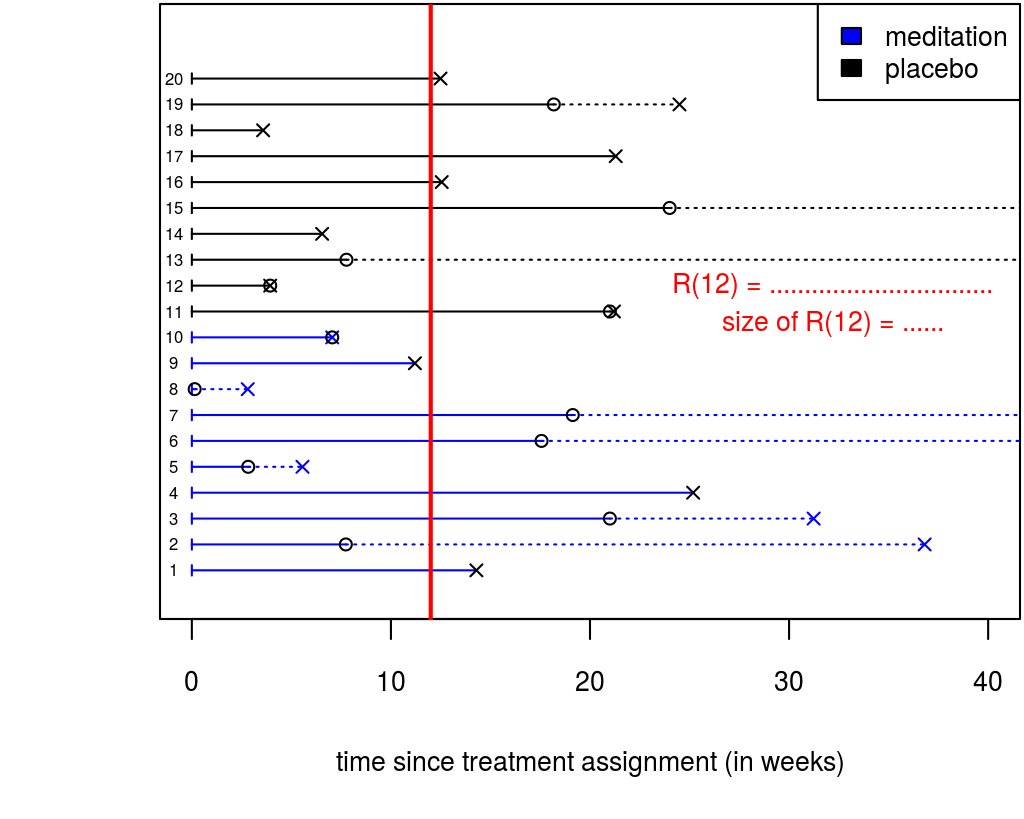
\includegraphics[height=0.8\textheight]{figs/risk_set_movie_4.png}
\end{center}

\textcolor{violet}{Pollev: \href{https://PollEv.com/free_text_polls/LvnDxrrdXRF0cixtAUMmz/respond}{link}} What is the size of the risk set at 12 weeks? \pause\textcolor{blue}{11}
\end{frame}

\begin{frame}
\frametitle{Risk set}
\begin{center}
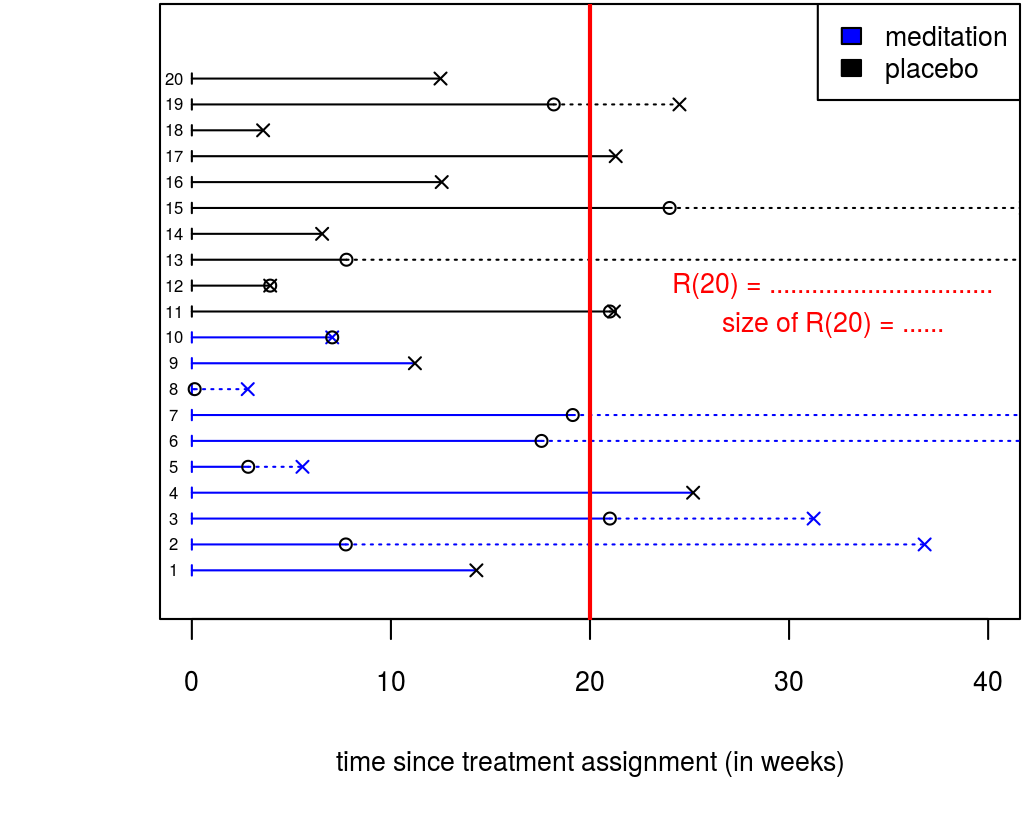
\includegraphics[height=0.8\textheight]{figs/risk_set_movie_5.png}
\end{center}

\textcolor{violet}{Pollev: \href{https://PollEv.com/free_text_polls/jVdeAH30QWlhfZZjPcUd1/respond}{link}} What is the size of the risk set at 20 weeks?  \pause\textcolor{blue}{5}
\end{frame}

\begin{frame}
\frametitle{Risk set}
\begin{center}
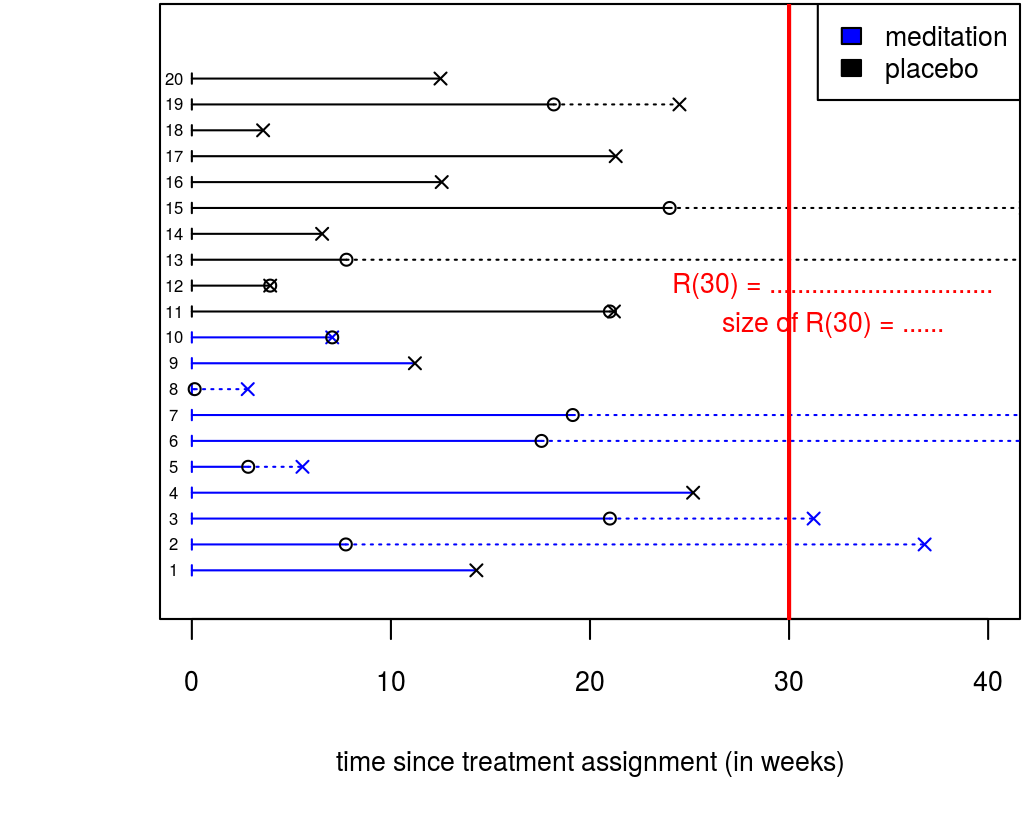
\includegraphics[height=0.8\textheight]{figs/risk_set_movie_6.png}
\end{center}

\textcolor{violet}{Pollev: \href{https://PollEv.com/free_text_polls/DTZO81Z0Lrl65SYGvMo6p/respond}{link}} What is the size of the risk set at 30 weeks?  \pause\textcolor{blue}{0}
\end{frame}

\begin{frame}
\frametitle{Assumptions}
The assumption of \textbf{independent (or uninformative) censoring} is critical to the vast majority of methods available in survival analysis.
\\ ~\ 

\textcolor{blue}{Independent censoring:} A participant's \textbf{time-to-event} and potential \textbf{censoring time} should be \textbf{independent} of one another.  
\\ ~\ 

What does that mean?   \textcolor{blue}{Individuals who are censored at time $t$ must be \textbf{similar} to those remaining in the risk set after time $t$.}  
\\ ~\ 

Independent censoring is a vital assumption, but unfortunately we can't do diagnostics or tests to see if it holds. 

\end{frame}

\begin{frame}{Assumptions}
	When is the independent censoring assumption reasonable? 
	
	\medskip
	
	\begin{itemize}
		\item Participants are censored because the study ended?   
		
		\medskip
		
		\item Participants exited the study because their panic disorder became disabling?  
		
		\medskip
		
		\item Participants exited the study because their panic disorder dissipated?  
		
		\medskip
		
		\item Participants exited the study because they moved to a different state?   
	\end{itemize}

\end{frame}


\begin{frame}{Assumptions}
	When is the independent censoring assumption reasonable? 
	
	\medskip
	
	\begin{itemize}
		\item Participants are censored because the study ended?   \textcolor{blue}{Yes!}
		
		\medskip
		
		\item Participants exited the study because their panic disorder became disabling?   \textcolor{red}{No!}
		
		\medskip
		
		\item Participants exited the study because their panic disorder dissipated?   \textcolor{red}{No!}
		
		\medskip
		
		\item Participants exited the study because they moved to a different state?   \textcolor{purple}{Maybe?}
	\end{itemize}
	
\end{frame}

\begin{frame}{Problems with means}
	
	\vspace{-7 mm}
	
	Fundamentally, a \textcolor{blue}{time-to-event} variable is \textcolor{red}{quantitative}, so you might think we'd be interested in the conditional mean.
	\\ ~\ 
	
	Unfortunately, with right censoring, we can't usually estimate the mean.  
	\begin{itemize}
		\medskip
		\item We need the full distribution of a variable to estimate the mean
		\medskip
		
		\item But we're missing some data in the right tail of the distribution (i.e., longer survival times)
	\end{itemize}
	\begin{figure}
		\centering
		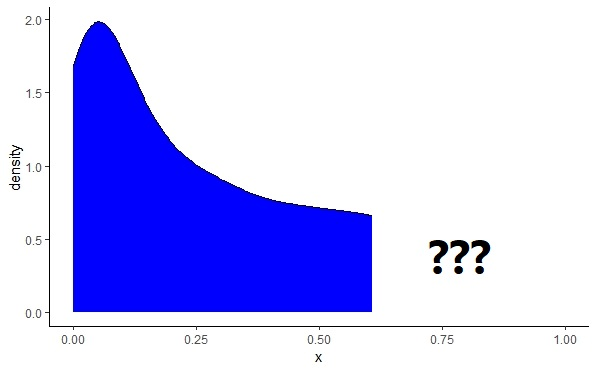
\includegraphics[scale = 0.3]{figs/mean_plot}
	\end{figure}
	\textbf{What can estimate instead?} 
\end{frame}
% key quantities: median, survival function, hazard function

\begin{frame}{Median survival time}
	If at least 50\% of our subjects experience the event, we can estimate the median time-to-event, often called the \textbf{\textcolor{blue}{median survival time}}.
	
	\bigskip
	
	\textbf{\textcolor{blue}{This will be the time when half of the participants have experienced the event and half have not.}}
	
	\bigskip 
	
	In order to estimate the median survival, we first need to estimate \textbf{\textcolor{blue}{the survival function}}.
\end{frame}


\begin{frame}
\frametitle{The survival function}
Suppose that $T$ is a continuous, time-to-event random variable (\textcolor{blue}{$T$ is our outcome of interest in survival analysis}).
\\ ~\ 

The \textbf{survival function}, $S$, is defined as $S(t) := P(T > t)$:  

\medskip

\begin{itemize}
\item \textcolor{blue}{$S(t) = $ proportion of the population with a time-to-event greater than $t$}  

\medskip

\item e.g.: if $S(20) = 0.37$, then approximately 37\% of the population will not experience a severe panic attack within the first 20 weeks  

\medskip

\item $S$ is \textcolor{blue}{non-increasing}, starts at 1 [i.e., $S(0) = 1$] and ends at 0 [i.e., $S(\infty) = 0$]
\end{itemize}
\end{frame}

\begin{frame}
\frametitle{The survival function}
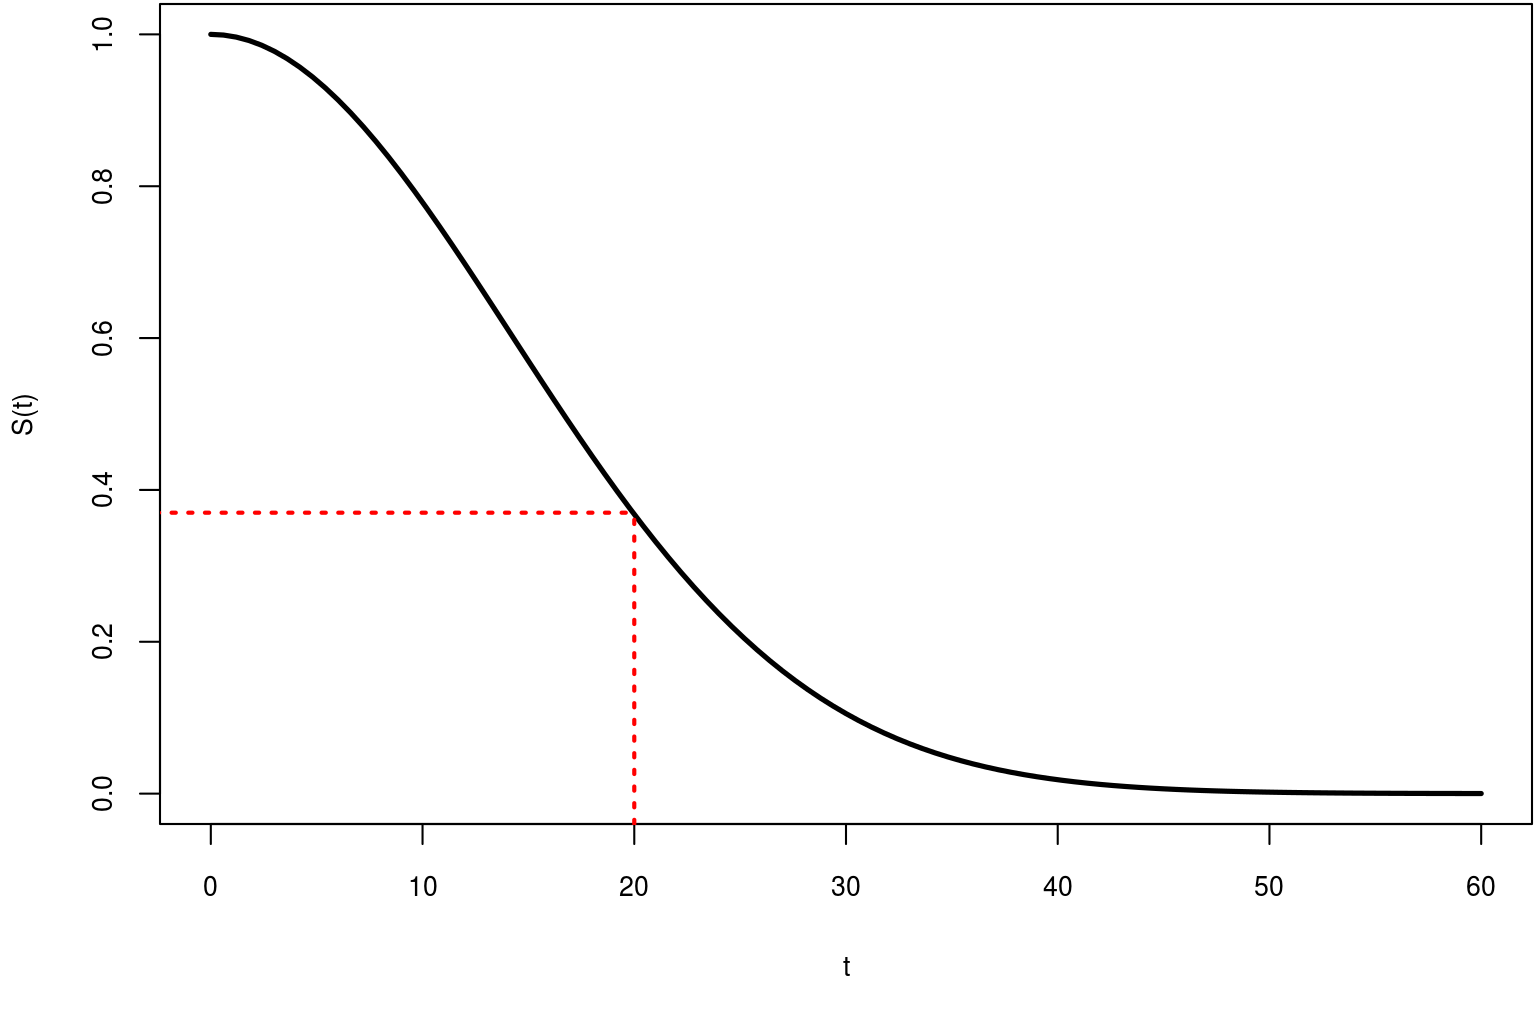
\includegraphics[height=0.8\textheight]{figs/survival_function.png}

\textcolor{violet}{Pollev: \href{https://PollEv.com/free_text_polls/f3xByyuUfSQMWmCKlR3j0/respond}{link}} What is S(10) (approximately)? \pause \textcolor{blue}{0.8 or 80\%}

\end{frame}

\begin{frame}
	\frametitle{The survival function}
	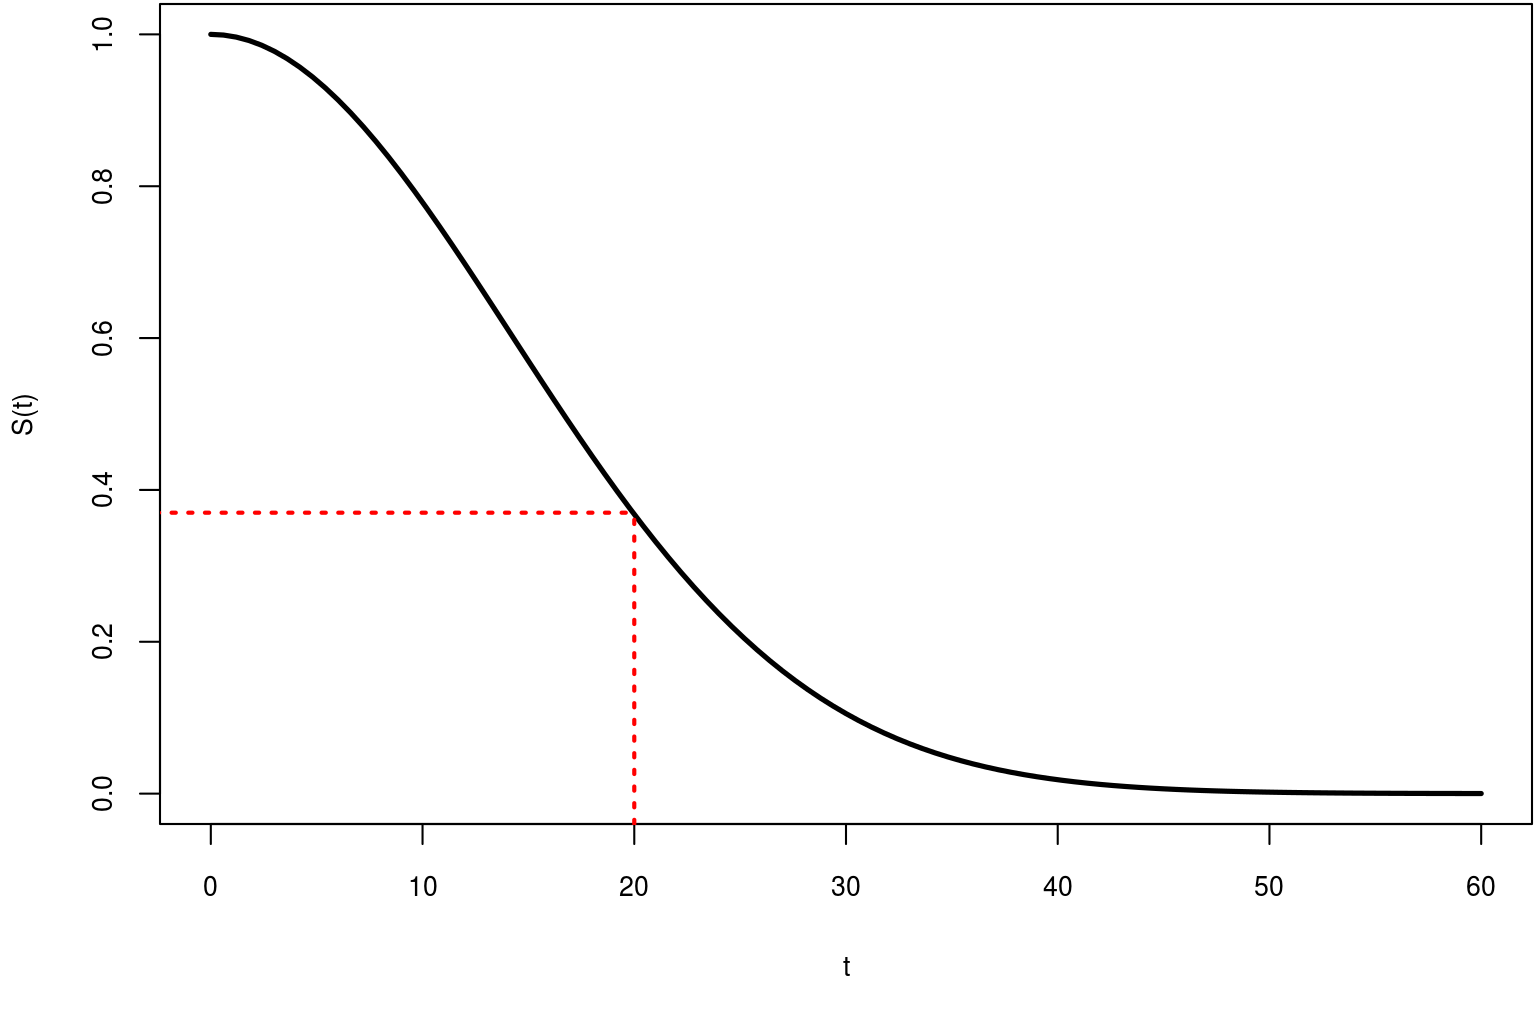
\includegraphics[height=0.8\textheight]{figs/survival_function.png}
	
	\textcolor{violet}{Pollev: \href{https://PollEv.com/free_text_polls/ncQUzw9d03Fbh7KIocDCw/respond}{link}} What is S(30) (approximately)? \pause \textcolor{blue}{0.1 or 10\%}
	
\end{frame}

\begin{frame}{Review: Incidence and prevalence}
	\begin{itemize}
		\item Incidence rate: number of people who develop a condition (incident events) per person per unit time
		
		\medskip
		
		\item Cumulative incidence: Fraction of individuals newly acquiring a condition over a specific time period
		
		\medskip
		
		\item Prevalence: fraction of individuals with the condition at a specific point in time
	\end{itemize}
\bigskip

	The \textcolor{blue}{\textbf{Hazard rate} $\mathbf{h(t)}$} is the \textcolor{blue}{\textit{instantaneous} incidence rate at time $t$}
\end{frame}


\begin{frame}
\frametitle{The hazard rate}

\vspace{-5 mm}

We observe $\Delta t$ time units starting at $t$. The incidence rate at $t$ is:
\smallskip
\color{blue}

\begin{align*}
 \frac{P(\text{having the event between }t\text{ and }t+\Delta t \mid \text{survived until time }t )}{1\text{ person }\times\Delta t}.
\end{align*}

\medskip
\color{black}


Which is:
\smallskip

\color{blue}
\begin{align*}
\frac{P(t \leq T < t + \Delta t \mid T \geq t)}{\Delta t}.
\end{align*}

\medskip

\color{black}

The \textbf{hazard rate} $\mathbf{h(t)}$ (instantaneous incidence rate) is

\smallskip
\color{blue}
\begin{align*}
h(t) = & \ \lim_{\Delta t \to 0} \frac{P(t \leq T < t + \Delta t \mid T \geq t)}{\Delta t}.
\end{align*} 

\end{frame}
 
 
 \begin{frame}
 	\frametitle{The hazard rate}
 	
 	
 	
\begin{itemize}
	
\item also called hazard function, failure rate

\medskip

\item In our panic attack example, $h(t)$ refers to the incidence rate of panic attacks at time $t$ after randomization 

	
	\medskip

\item $h(t)\times \Delta t$ approximates the probability that $T$ is in the interval $[t, t + \Delta t)$ given $T \geq t$

\medskip

\item $h(t)$ is between 0 and $\infty$





\end{itemize}


\bigskip

The \textcolor{blue}{\textbf{cumulative hazard function}} $H$ is given by $H(t) := \int_0^t h(u) du$.

\medskip

\begin{itemize}
	\item Since $h(t)$ is strictly positive, $H(t)$ is an \textcolor{blue}{increasing} function
\end{itemize}

\end{frame}



\begin{frame}
\frametitle{Key quantities in survival analysis}
Most methods in survival analysis focus on modeling and/or estimating either the \textcolor{blue}{survival function} or the \textcolor{blue}{hazard rate}.
\\ ~\ 

The hazard rate, while pretty unintuitive, has the desirable property that it can be \textcolor{blue}{easily estimated using right-censored data}.

\medskip

\begin{itemize}
	\item You can show this using rules of probability. If you're curious I can talk in office hours!
\end{itemize}
\end{frame}

\begin{frame}
\frametitle{Thinking about hazards}
What shape do we expect the hazard function to have? \textcolor{red}{It depends...}
\begin{enumerate}[(a)]
\item survival from surgery until death due to complications
\item survival from onset of a progressive disease
\item the time before a radioactive atom disintegrates
\item an individual's total lifetime
\end{enumerate}
\begin{center}
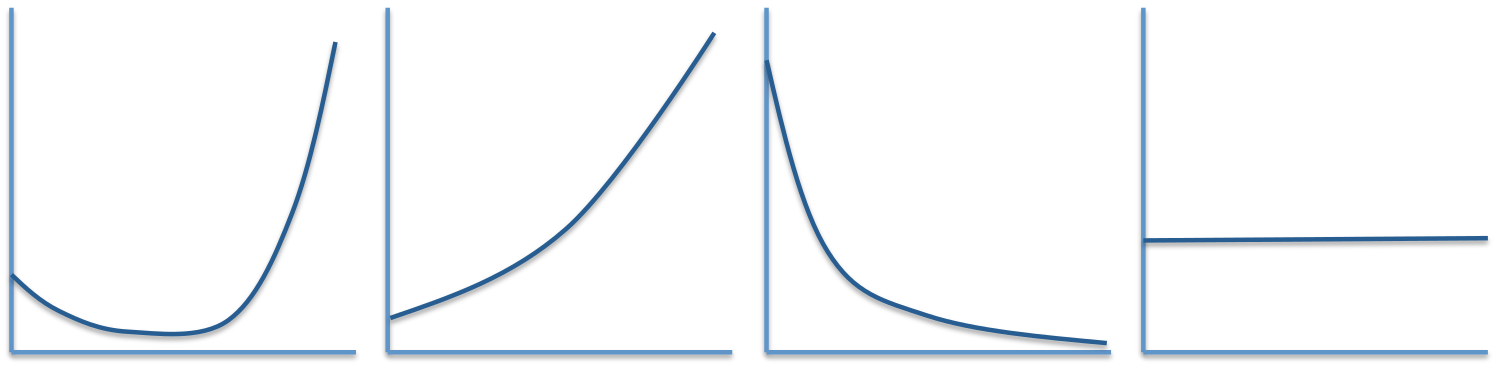
\includegraphics[width = 0.9\textwidth]{figs/hazard_examples.png}

\underline{\,\phantom{right}\,} \hspace{1.5cm} \underline{\,\phantom{right}\,} \hspace{1.5cm} \underline{\,\phantom{right}\,} \hspace{1.5cm} \underline{\,\phantom{right}\,}
\end{center}
\end{frame}

\begin{frame}
	\frametitle{Thinking about hazards}
	What shape do we expect the hazard function to have? \textcolor{red}{It depends...}
	\begin{enumerate}[(a)]
		\item survival from surgery until death due to complications
		\item survival from onset of a progressive disease
		\item the time before a radioactive atom disintegrates
		\item an individual's total lifetime
	\end{enumerate}
	\begin{center}
		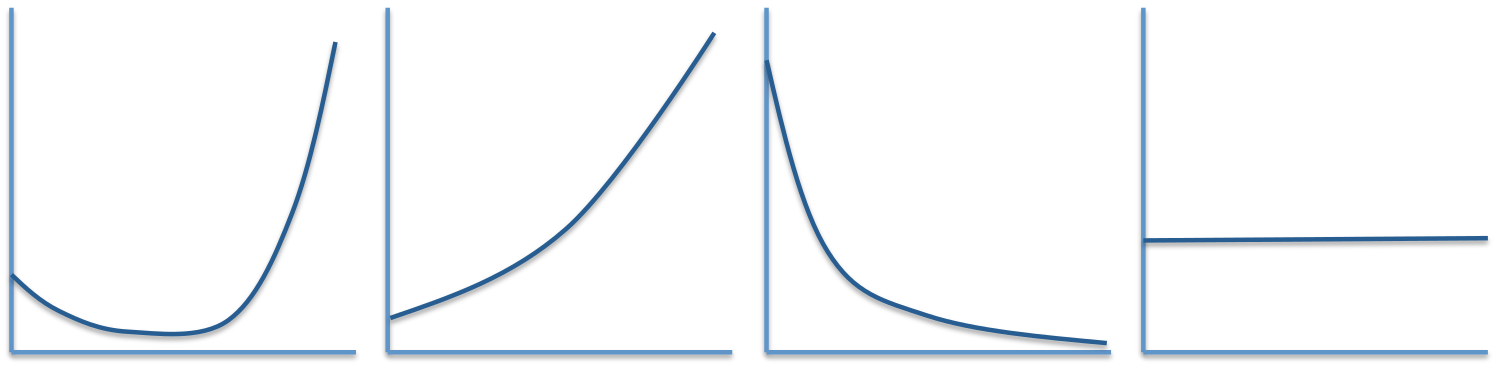
\includegraphics[width = 0.9\textwidth]{figs/hazard_examples.png}
		
		(d) \hspace{1.5cm} (b) \hspace{1.5cm} (a) \hspace{1.5cm} (c)
	\end{center}
\end{frame}

\begin{frame}{Characteristics of survival data: summary}
	\begin{itemize}
		\item In survival analysis we study variables representing the time to some event occurring.
		
		\medskip
		
		\item Survival data are generally subject to being right-censored.
		
		\medskip
		
		\item Simply ignoring censored data is not a good idea!
		
		\medskip
		
		\item Most methods rely on the assumption of \textcolor{blue}{independent censoring}.
		
		\medskip
		
		\item Key quantities: the risk set, the hazard function, the survival function
	\end{itemize}
\end{frame}


\section{Kaplan-Meier and the log rank test}

\begin{frame}
\frametitle{Reframing survival data}

\vspace{-5 mm}

As we think about estimation, it'll be useful to change notation.
\\ ~\ 

For participant $i$, denote by $T_i$ \textbf{the time to event} and by $C_i$ \textbf{the time to censoring}.   
\\ ~\ 

We cannot observe both $T_i$ and $C_i$ -- instead, we observe a pair $(Y_i, \Delta_i)$, where   
\begin{itemize}
	\medskip
\item $Y_i := \min(T_i, C_i)$ is the \textbf{observed follow-up time}  

\medskip
\item $\Delta_i = I(T_i \leq C_i)$ is the \textbf{event indicator}, equal to 1 if event is observed and zero if observation censored
\end{itemize}
\medskip

\textbf{Question:} In this new notation, how would we represent the data $\{7.5, 16.6+, 13.5+, 7.4, 14.2\}$?  
\[\{(7.5, 1), (16.6, 0), (13.5, 0), (7.4, 1), (14.2, 1)\}.\]
\end{frame}

\begin{frame}
\frametitle{Estimating survival function}

\vspace{-5 mm}

Let's start by \textbf{estimating the survival probability at time $t$}: $S(t) = P(T > t)$.
\\ ~\ 

If we observed actual survival times $T_1, T_2, \dots, T_n$, we could have
\begin{align*}
\widehat{S}(t)=\frac{1}{n}\sum_{i=1}^n I(T_i > t)
\end{align*}
 (in other words, just count how many people made it past time $t$ without an event). 
 
 \medskip
 
 This is a \textcolor{blue}{nonparametric} estimator; we do not have to assume a parametric model for the true survival distribution, unlike with linear regression, for example, where we assumed a linear model. 
\\ ~\ 

Can we use this estimator in practice?   \textbf{\textcolor{red}{No, since we do not see $T_i$ for participants who are censored!}}
\end{frame}

\begin{frame}
\frametitle{Kaplan-Meier estimation of survival function}
	What about using the observed follow-up times?
	\begin{align*}
		\frac{1}{n}\sum_{i=1}^{n}I(Y_i > t)
	\end{align*}
	
	where $Y_i = \min(T_i,C_i)$
	
	\bigskip
	
	\textcolor{violet}{Pollev: \href{https://PollEv.com/multiple_choice_polls/buQTHdd72xMJq25jNb3Y3/respond}{link}} Would this be an \textcolor{blue}{overestimate} or \textcolor{red}{underestimate} of $P(T > t)$?  \pause 
	\\ ~\ 
	
	\textbf{Answer:} It would be an \textcolor{red}{underestimate}. Some people would have survived past time $t$, had they not been censored. 
	
	\medskip
	
	(If it helps to think mathematically, we know that $Y_i \leq T_i$ for all $i$, so using $Y_i$ in place of $T_i$ can only make our estimate smaller.)
\end{frame}


\begin{frame}{Review: Conditional and joint probability}
	We will need to use the following rule. For events $A$ and $B$
	\begin{itemize}
		\item Let \textcolor{blue}{$P(A, B) = P(A \text{ and } B)$} be the \textcolor{blue}{joint probability of $A$ and $B$} (probability that both events occur)
		
		\medskip
		
		\item Let \textcolor{blue}{$P(A \mid B)$} be the \textcolor{blue}{conditional probability of $A$ given $B$} (probability that $A$ occurs given that $B$ has occurred)
	\end{itemize}

\bigskip

	It is a fact that
	\begin{align*}
		\textcolor{blue}{P(A, B) = P(A \mid B)P(B).}
	\end{align*}
\end{frame}

\begin{frame}{Estimating the Survival Function}
	
	Using this, for $t_2<t_3$:
	
	\begin{align*}
	S(t_3)=P(T>t_3)
	\end{align*}
	
	Then, if we survive till $t_3$ we've already survived till $t_2$, so:
	
		\begin{align*}
	S(t_3)=P(T>t_3,T > t_2)
	\end{align*}
	
	Then, using the fact about conditional probability:
	
	\begin{align*}
	S(t_3)=P(T>t_3|T>t_2)\textcolor{blue}{P(T>t_2)}
	\end{align*}
	
	
	Which is:
	
		\begin{align*}
	S(t_3)=P(T>t_3|T>t_2)\textcolor{blue}{S(t_2)}
	\end{align*}
	
\end{frame}

\begin{frame}{Estimating the Survival Function}
	
	We can do this multiple times. Now say we also have $t_1<t_2$:
	
	\begin{align*}
	S(t_3)=P(T>t_3|T>t_2)\textcolor{blue}{P(T>t_2)}
	\end{align*}
	
	\begin{align*}
	S(t_3)=P(T>t_3|T>t_2)\textcolor{blue}{P(T>t_2,T>t_1)}
	\end{align*}
	
	
	Using our rule again:
	
	\begin{align*}
	S(t_3)=P(T>t_3|T>t_2)P(T>t_2|T>t_1)\textcolor{blue}{P(T > t_1)}
	\end{align*}
	
	\begin{align*}
	S(t_3)=P(T>t_3|T>t_2)P(T>t_2|T>t_1)\textcolor{blue}{S(t_1)}
	\end{align*}
	
\end{frame}

\begin{frame}{Estimating the Survival Function}
	
	\textcolor{blue}{We can do this many, many, times until we get to time 0}
	
		\begin{align*}
	S(t_{10})=P(T>t_{10}|T>t_9)P(T>t_9|T>t_8)...P(T>t_1|T>0)S(0)
	\end{align*}
	
	\medskip
	
	In words, the probability that we survive past time ten is the probability that we survive past time 10 given that we've survived past time 9, times the probability that we survive past time 9 given that we've survived past time 8, etc., times the probability that we survive past time 1 given that we've survived past time 0, times the probability of survival at time 0.
	
\end{frame}

\begin{frame}{Estimating the Survival Function}
	How does this help us estimate survival?
	

	
	\medskip
	
		\[\textcolor{blue}{P(T>t_{2}|T>t_1)\approx \frac{\text{\# people who survived at }t_2}{\text{\# people alive and under observation at }t_2 }}\]
	
	in other words

	\medskip
	
	\[\textcolor{blue}{P(T>t_{2}|T>t_1)\approx \frac{\text{\# people who survived at }t_2}{\text{size of risk set at }t_2 }}\]
	
	also
	
	\[\textcolor{blue}{S(0)=1}\]
	
	
\end{frame}

\begin{frame}{Estimating the Survival Function}
	Putting this all together, we get the \textcolor{blue}{\textbf{Kaplan-Meier estimator}}:
	
	
	
	\medskip
	
	\small
	
	\begin{align*}
	\widehat{S}(t_{10})=\frac{\text{\# people who survived at }t_{10}}{\text{size of risk set at }t_{10}}\times \frac{\text{\# people who survived at }t_9}{\text{size of risk set at }t_9 }\times ...
	\end{align*}
	
	\begin{align*}
	\textcolor{white}{\widehat{S}(t_{10})=}...\times \frac{\text{\# people who survived at }t_1}{\text{size of risk set at }t_1 }\times 1\textcolor{white}{\times \frac{\text{\# people who survived at }t_9}{\text{size of risk set at }t_9 }}
	\end{align*}
	
	\normalsize
	
	\bigskip
	
	\textcolor{blue}{Question:} Which times do we use?
	
	\medskip
	
	All of the observed follow-up times $y$ in the data!

	
\end{frame}


\begin{frame}
	\frametitle{Kaplan-Meier estimation of survival function}
	\vspace{-0.8cm}
	Denote by $t_1 < t_2 < \dots < t_m$ the ordered, distinct, observed times (event or censoring). (\textbf{Question}: When is $m$ equal to $n$, the sample size?   \textbf{Answer}: When all the times are unique (no ties).)  
	\\ ~\
	
	Also, denote: 
	\begin{align*}
	d_k = & \ \text{\# of events having occurred at time $t_k$} \\
	n_k = & \ \text{\# of individuals \textbf{at risk} at time $t_k$}
	\end{align*}
	\textcolor{blue}{Suppose the data are $\{4, 5, 5+, 8, 12+, 13, 18+, 23, 23, 30\}$}.  
	
	\begin{center}
		\begin{tabular}{|c|c|c|c|}
			\hline
			$k$ & time $t_k$ & $d_k$ & $n_k$ \\
			\hline
			1 & 4 & 1 & 10 \\
			2& 5 & 1 & 9 \\
			3& 8 & 1 & 7 \\
			4&12 & 0 & 6 \\
			5&13 & 1 & 5 \\
			6&18 & 0 & 4 \\
			7&23 & 2 & 3 \\
			8&30 & 1 & 1 \\
			\hline
		\end{tabular}
	\end{center}
\end{frame}

\begin{frame}
\frametitle{Kaplan-Meier estimation of survival function}

	\vspace{-5 mm}

\textcolor{blue}{What is $\widehat{S}(4)$?}

\medskip

\begin{columns}
	\begin{column}{0.3\textwidth}
		\begin{center}
\begin{tabular}{|c|c|c|c|}
	\hline
	$k$ & $t_k$ & $d_k$ & $n_k$ \\
	\hline
	1 & 4 & 1 & 10 \\
	2& 5 & 1 & 9 \\
	3& 8 & 1 & 7 \\
	4&12 & 0 & 6 \\
	5&13 & 1 & 5 \\
	6&18 & 0 & 4 \\
	7&23 & 2 & 3 \\
	8&30 & 1 & 1 \\
	\hline
\end{tabular}
	\end{center}
	\end{column}
	\begin{column}{0.7\textwidth}  %%<--- here
		\begin{align*}
			P(T > t_1) &= P(T > t_1, T > 0) \\
			&= P(T > t_1 \mid T > 0)P(T > 0)
		\end{align*}
		How many people made it to \textbf{at least} $t_1$ without an event?   \textcolor{blue}{10/10}
		\\ ~\ 
		
		Among those who make it to at least $t_1$ without an event, how many \textbf{survive past} $t_1$?   \textcolor{blue}{9/10} 
	\end{column}
\end{columns}
\vspace{0.5cm}
So our estimate of $S(4) = P(T > t_1)$ is \textcolor{blue}{$\frac{9}{10} \times \frac{10}{10} = 0.9$}.
\end{frame}

\begin{frame}
	\frametitle{Kaplan-Meier estimation of survival function}
	
		\vspace{-5 mm}
	
	\textcolor{blue}{What is $\widehat{S}(5)$?}
	
	\medskip
	
	\begin{columns}
		\begin{column}{0.3\textwidth}
			\begin{center}
				\begin{tabular}{|c|c|c|c|}
					\hline
					$k$ & $t_k$ & $d_k$ & $n_k$ \\
					\hline
					1 & 4 & 1 & 10 \\
					2& 5 & 1 & 9 \\
					3& 8 & 1 & 7 \\
					4&12 & 0 & 6 \\
					5&13 & 1 & 5 \\
					6&18 & 0 & 4 \\
					7&23 & 2 & 3 \\
					8&30 & 1 & 1 \\
					\hline
				\end{tabular}
			\end{center}
		\end{column}
		\begin{column}{0.7\textwidth}  %%<--- here
			\begin{align*}
			P(T > t_2) &= P(T > t_2, T > t_1) \\
			&= P(T > t_2 \mid T > t_1)P(T > t_1)
			\end{align*}
				We already have an estimate of $P(T > t_1)$: \textcolor{blue}{0.9}  
			\\ ~\ 
			
			\textcolor{violet}{Pollev: \href{https://PollEv.com/free_text_polls/0ZMy8Tg91FRE7uYQeUDMl/respond}{link} }Among those who make it to at least $t_2$ without an event, how many \textbf{survive past} $t_2$? \pause   \textcolor{blue}{8/9} 
		\end{column}
	\end{columns}
	\vspace{0.5cm}
	So our estimate of $S(5) = P(T > t_2)$ is \textcolor{blue}{$\frac{8}{9} \times \frac{9}{10} = 0.8$}.
\end{frame}

\begin{frame}
	\frametitle{Kaplan-Meier estimation of survival function}
	
	\vspace{-5 mm}
	
	\textcolor{blue}{What is $\widehat{S}(8)$?}
	
	\medskip
	
	\begin{columns}
		\begin{column}{0.3\textwidth}
			\begin{center}
				\begin{tabular}{|c|c|c|c|}
					\hline
					$k$ & $t_k$ & $d_k$ & $n_k$ \\
					\hline
					1 & 4 & 1 & 10 \\
					2& 5 & 1 & 9 \\
					3& 8 & 1 & 7 \\
					4&12 & 0 & 6 \\
					5&13 & 1 & 5 \\
					6&18 & 0 & 4 \\
					7&23 & 2 & 3 \\
					8&30 & 1 & 1 \\
					\hline
				\end{tabular}
			\end{center}
		\end{column}
		\begin{column}{0.7\textwidth}  %%<--- here
			\begin{align*}
			P(T > t_3) &= P(T > t_3, T > t_2) \\
			&= P(T > t_3 \mid T > t_2)P(T > t_2)
			\end{align*}
			We already have an estimate of $P(T > t_2)$: \textcolor{blue}{0.8}  
			\\ ~\ 
			
			\textcolor{violet}{Pollev: \href{https://PollEv.com/free_text_polls/oxjKMRbHncKvL4aoSLfE3/respond}{link} }Among those who make it to at least $t_3$ without an event, how many \textbf{survive past} $t_3$? \pause   \textcolor{blue}{6/7} 
		\end{column}
	\end{columns}
	\vspace{0.5cm}
	So our estimate of $S(8) = P(T > t_3)$ is \textcolor{blue}{$\frac{6}{7} \times \frac{8}{10} = 0.686$}.
	
	\medskip
	
	 \textcolor{red}{Note that because of censoring, we don't know if the person censored at $t = 5$ had an event before $t = 8$. But since \textbf{we assume independent censoring}, we treat the people at risk at $t = 8$ \textbf{as if they are representative of the person censored} at $t = 5$.}   
\end{frame}




\begin{frame}
\frametitle{Kaplan-Meier estimation of survival function}

\vspace{-5 mm}

Continuing in this fashion yields the \textbf{Kaplan-Meier} estimator: 
\begin{align*}
\widehat{S}(t) := \prod_{k: t_k \leq t} \left(1 - \frac{d_k}{n_k} \right) = \prod_{k: t_k \leq t} \left(1 - \frac{\text{\# of events at $t_k$}}{\text{\# at risk at $t_k$}} \right) .
\end{align*}

If any participant is censored at the final observed time, we consider $\widehat{S}(t)$ to be undefined for all later times. 

\medskip


\begin{itemize}
\item $\widehat{S}(t) = 1$ until the first event time 
\medskip

\item $\widehat{S}$ is a non-increasing function. Why?  

\medskip
\item $\widehat{S}$ drops to zero at the last observed time only if the last observed time is all events (not censoring)  

\medskip
\item $\widehat{S}$ is nonparametric, meaning we assume independent censoring but do not assume a model

\medskip
\item the KM estimator only changes at observed event times, and is constant (flat) between observed times  
\end{itemize}
\end{frame}

\begin{frame}
\frametitle{Kaplan-Meier estimation of survival function}

\begin{tabular}{|c|c|c|c|c|c|}
\hline
time $t_k$ & $d_k$ & $n_k$ & $d_k/n_k$ & $1 - d_k/n_k$ & $\widehat{S}(t_k)$ \\
\hline
4 & 1 & 10 & 0.1 & \textcolor{blue}{0.9} & $1 \times \textcolor{blue}{0.9} = \textcolor{blue}{0.9}$\\
5 & 1 & 9 & 0.1111 & \textcolor{blue}{0.8888} & $0.9 \times \textcolor{blue}{0.8888} = \textcolor{blue}{0.8}$ \\
8 & 1 & 7 & 0.1429 & \textcolor{blue}{0.8571} & $0.8 \times \textcolor{blue}{0.8571} = \textcolor{blue}{0.6857}$\\
12 & 0 & 6 & 0 & \textcolor{blue}{1} & $0.6857 \times \textcolor{blue}{1} = \textcolor{blue}{0.6857}$\\
13 & 1 & 5 & 0.2 & \textcolor{blue}{0.8} & $0.6857 \times \textcolor{blue}{0.8} = \textcolor{blue}{0.5486}$\\
18 & 0 & 4 & 0 & \textcolor{blue}{1} & $0.5846 \times \textcolor{blue}{1} = \textcolor{blue}{0.5486}$\\
23 & 2 & 3 & 0.666 & \textcolor{blue}{0.3333} & $0.5486 \times \textcolor{blue}{0.3333} = \textcolor{blue}{0.1829}$\\
30 & 1 & 1 & 1 & \textcolor{blue}{0} & $0.1829 \times \textcolor{blue}{0} = \textcolor{blue}{0}$\\
\hline
\end{tabular}
\end{frame}

\begin{frame}
\frametitle{Kaplan-Meier estimation of survival function}

\centering
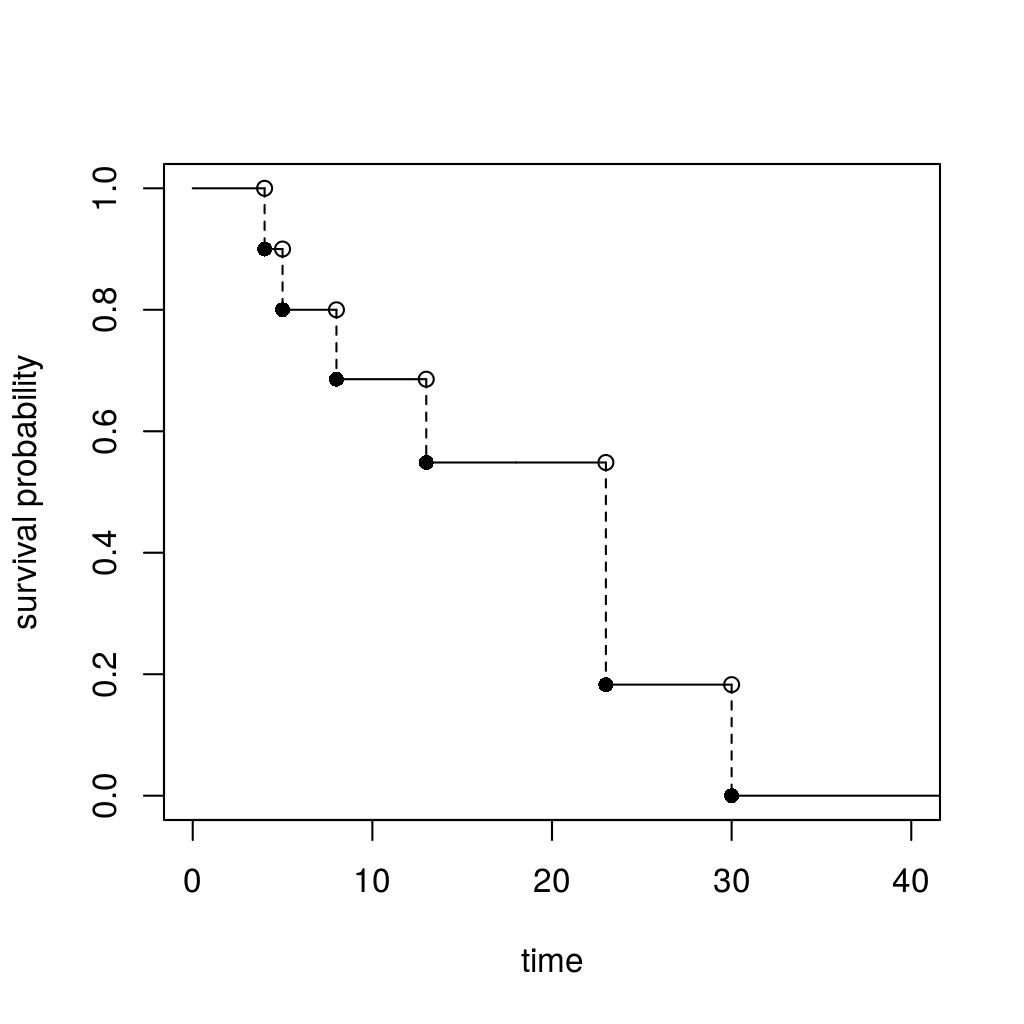
\includegraphics[width=0.7\textwidth]{figs/km_small_example.png}
\end{frame}

\begin{frame}{Another framing of Kaplan-Meier}
	You could also think about Kaplan-Meier as a ``redistribution to the right" estimator, which may be more intuitive for some.
	
	\medskip 
	\begin{enumerate}
		\item Arrange the $n$ observed times (events or censorings) in increasing order (if there are ties, censorings go after events)
		
		\medskip
		
		\item Assign weight $1/n$ to each observation
		
		\medskip
		
		\item Moving from left to right, each time you encounter a censored observation, \textcolor{blue}{redistribute} its weight evenly over all times to its right (events and censoring times)
		
		\medskip
		
		\item Approximate the survival probability at each time point by adding up remaining weights at that time point
	\end{enumerate}
\end{frame}

\begin{frame}{Redistribute to the right}
	
	\vspace{-5 mm}
	
	\begin{itemize}
		\item Redistribute weight at each censoring time
		
		\medskip
		\item Add up remaining weights at each observed event time
		
		\smallskip
	\end{itemize}
	\begin{footnotesize}
		\begin{center}
		\begin{tabular}{|c|c|c|c|c|}
			\hline
			$t_k$ & $d_k$ & $n_k$ & Weight per obs. & Remaining weight = $\widehat{S}(t_k)$ \\
			\hline
			4 & 1 & 10 & $\frac{1}{10} = 0.1$ & $9\times 0.1= 0.9$\\
			5 & 1 & 9 & & \\
			8 & 1 & 7 & & \\
			12 & 0 & 6 & & \\
			13 & 1 & 5 & & \\
			18 & 0 & 4 & & \\
			23 & 2 & 3 & & \\
			30 & 1 & 1 & & \\
			\hline
		\end{tabular}
	\end{center}
	\end{footnotesize}
\medskip

	\begin{enumerate}
		\item \textcolor{blue}{no censoring --- no weight redistribution}
		
		\medskip
		
		\item \textcolor{blue}{9 subjects remaining after observed event}
	\end{enumerate}
\end{frame}

\begin{frame}{Redistribute to the right}
	
	\vspace{-5 mm}
	
	
	\begin{itemize}
		\item Redistribute weight at each censoring time
		
		\medskip
		
		\item Add up remaining weights at each observed event time
		
		\smallskip
		
	\end{itemize}
	\begin{footnotesize}
		\begin{center}
		\begin{tabular}{|c|c|c|c|c|}
			\hline
			$t_k$ & $d_k$ & $n_k$ & Weight per obs. & Remaining weight = $\widehat{S}(t_k)$ \\
			\hline
			4 & 1 & 10 & $\frac{1}{10} = 0.1$ & $9\times 0.1= 0.9$\\
			5 & 1 & 9 & $0.1$ &  $8\times 0.1= 0.8$  \\
			8 & 1 & 7 & & \\
			12 & 0 & 6 & & \\
			13 & 1 & 5 & & \\
			18 & 0 & 4 & & \\
			23 & 2 & 3 & & \\
			30 & 1 & 1 & & \\
			\hline
		\end{tabular}
	\end{center}
	\end{footnotesize}

\medskip

	\begin{enumerate}
		\item \textcolor{blue}{no censoring --- no weight redistribution}
		
		\medskip
		
		\item \textcolor{blue}{8 subjects remaining after observed event}
	\end{enumerate}
\end{frame}

\begin{frame}{Redistribute to the right}
	
	\vspace{-5 mm}
	
	\begin{itemize}
		\item Redistribute weight at each censoring time
		
		\medskip
		
		\item Add up remaining weights at each observed event time
		
		\smallskip
		
	\end{itemize}
	\begin{footnotesize}
		\begin{center}
		\begin{tabular}{|c|c|c|c|c|}
			\hline
			$t_k$ & $d_k$ & $n_k$ & Weight per obs. & Remaining weight = $\widehat{S}(t_k)$ \\
			\hline
			4 & 1 & 10 & $\frac{1}{10} = 0.1$ & $9\times 0.1= 0.9$\\
			5 & 1 & 9 & $0.1$ &  $8\times 0.1= 0.8$  \\
			8 & 1 & 7 & $0.1 + (0.1\times \frac{1}{7}) = 0.1143$ & $7 \times 0.1143 = 0.6857$\\
			12 & 0 & 6 & & \\
			13 & 1 & 5 & & \\
			18 & 0 & 4 & & \\
			23 & 2 & 3 & & \\
			30 & 1 & 1 & & \\
			\hline
		\end{tabular}
	\end{center}
	\end{footnotesize}

\medskip
	\begin{enumerate}
		\item \textcolor{blue}{1 censored --- redistribute weight over remaining 7}
		
		\medskip
		
		\item \textcolor{blue}{7 subjects remaining after observed event}
	\end{enumerate}
\end{frame}

\begin{frame}{Redistribute to the right}
	
\vspace{-5 mm}	
	
	\begin{itemize}
		\item Redistribute weight at each censoring time
		
		\medskip
		
		\item Add up remaining weights at each observed event time
	\end{itemize}

\smallskip

	\begin{footnotesize}
		\begin{center}
		\begin{tabular}{|c|c|c|c|c|}
			\hline
			$t_k$ & $d_k$ & $n_k$ & Weight per obs. & Remaining weight = $\widehat{S}(t_k)$ \\
			\hline
			4 & 1 & 10 & $\frac{1}{10} = 0.1$ & $9\times 0.1= 0.9$\\
			5 & 1 & 9 & $0.1$ &  $8\times 0.1= 0.8$  \\
			8 & 1 & 7 & $0.1 + (0.1\times \frac{1}{7}) = 0.1143$ & $7 \times 0.1143 = 0.6857$\\
			12 & 0 & 6 & $0.1143 +  (0.1143\times\frac{1}{5}) = 0.1371$ &  0.6857\\
			13 & 1 & 5 & & \\
			18 & 0 & 4 & & \\
			23 & 2 & 3 & & \\
			30 & 1 & 1 & & \\
			\hline
		\end{tabular}
	\end{center}
	\end{footnotesize}

\medskip
	\begin{enumerate}
		\item \textcolor{blue}{1 censored --- redistribute weight over remaining 5}
		
		\medskip
		
		\item \textcolor{blue}{no observed events}
	\end{enumerate}
\end{frame}

\begin{frame}{Redistribute to the right}
	
	\vspace{-5 mm}
	
	\begin{itemize}
		\item Redistribute weight at each censoring time
		
		\medskip
		
		\item Add up remaining weights at each observed event time
	\end{itemize}

\smallskip

	\begin{footnotesize}
		\begin{center}
		\begin{tabular}{|c|c|c|c|c|}
			\hline
			$t_k$ & $d_k$ & $n_k$ & Weight per obs. & Remaining weight = $\widehat{S}(t_k)$ \\
			\hline
			4 & 1 & 10 & $\frac{1}{10} = 0.1$ & $9\times 0.1= 0.9$\\
			5 & 1 & 9 & $0.1$ &  $8\times 0.1= 0.8$  \\
			8 & 1 & 7 & $0.1 + (0.1\times \frac{1}{7}) = 0.1143$ & $7 \times 0.1143 = 0.6857$\\
			12 & 0 & 6 & $0.1143 +  (0.1143\times\frac{1}{5}) = 0.1371$ &  0.6857\\
			13 & 1 & 5 & 0.1371 & $4 \times 0.1371 =0.5486 $\\
			18 & 0 & 4 & & \\
			23 & 2 & 3 & & \\
			30 & 1 & 1 & & \\
			\hline
		\end{tabular}
	\end{center}
	\end{footnotesize}
\medskip

	\begin{enumerate}
		\item \textcolor{blue}{no censoring --- no weight redistribution}
		
		\medskip
		
		\item \textcolor{blue}{4 subjects remaining after observed event}
	\end{enumerate}
\end{frame}

\begin{frame}{Redistribute to the right}
	
	\vspace{-5 mm}
	
	\begin{itemize}
		\item Redistribute weight at each censoring time
		
		\medskip
		
		\item Add up remaining weights at each observed event time
	\end{itemize}

\smallskip

	\begin{footnotesize}
		\begin{center}
		\begin{tabular}{|c|c|c|c|c|}
			\hline
			$t_k$ & $d_k$ & $n_k$ & Weight per obs. & Remaining weight = $\widehat{S}(t_k)$ \\
			\hline
			4 & 1 & 10 & $\frac{1}{10} = 0.1$ & $9\times 0.1= 0.9$\\
			5 & 1 & 9 & $0.1$ &  $8\times 0.1= 0.8$  \\
			8 & 1 & 7 & $0.1 + (0.1\times \frac{1}{7}) = 0.1143$ & $7 \times 0.1143 = 0.6857$\\
			12 & 0 & 6 & $0.1143 +  (0.1143\times\frac{1}{5}) = 0.1371$ &  0.6857\\
			13 & 1 & 5 & 0.1371 & $4 \times 0.1371 =0.5486 $\\
			18 & 0 & 4 & $0.1371 + (0.1371\times \frac{1}{3}) = 0.1829$ & 0.5486\\
			23 & 2 & 3 & & \\
			30 & 1 & 1 & & \\
			\hline
		\end{tabular}
	\end{center}
	\end{footnotesize}

\medskip
	\begin{enumerate}
		\item \textcolor{blue}{1 censored --- redistribute weight over remaining 3}
		
		\medskip
		
		\item \textcolor{blue}{no observed events}
	\end{enumerate}
\end{frame}

\begin{frame}{Redistribute to the right}
	
	
	\vspace{-5 mm}
	
	\begin{itemize}
		\item Redistribute weight at each censoring time
		
		\medskip
		
		\item Add up remaining weights at each observed event time
	\end{itemize}

\smallskip


	\begin{footnotesize}
		\begin{center}
		\begin{tabular}{|c|c|c|c|c|}
			\hline
			$t_k$ & $d_k$ & $n_k$ & Weight per obs. & Remaining weight = $\widehat{S}(t_k)$ \\
			\hline
			4 & 1 & 10 & $\frac{1}{10} = 0.1$ & $9\times 0.1= 0.9$\\
			5 & 1 & 9 & $0.1$ &  $8\times 0.1= 0.8$  \\
			8 & 1 & 7 & $0.1 + (0.1\times \frac{1}{7}) = 0.1143$ & $7 \times 0.1143 = 0.6857$\\
			12 & 0 & 6 & $0.1143 +  (0.1143\times\frac{1}{5}) = 0.1371$ &  0.6857\\
			13 & 1 & 5 & 0.1371 & $4 \times 0.1371 =0.5486 $\\
			18 & 0 & 4 & $0.1371 + (0.1371\times \frac{1}{3}) = 0.1829$ & 0.5486\\
			23 & 2 & 3 & 0.1829&  $1 \times 0.1829 = 0.1829$\\
			30 & 1 & 1 & & \\
			\hline
		\end{tabular}
	\end{center}
	\end{footnotesize}

\medskip

	\begin{enumerate}
		\item \textcolor{blue}{no censoring --- no weight redistribution}
		
		\medskip
		
		\item \textcolor{blue}{1 subject remaining after 2 observed events}
	\end{enumerate}
\end{frame}

\begin{frame}{Redistribute to the right}
	
	\vspace{-5 mm}
	
\begin{itemize}
	\item Redistribute weight at each censoring time
	
	\medskip
	
	\item Add up remaining weights at each observed event time
\end{itemize}

\smallskip

		\begin{footnotesize}
			\begin{center}
		\begin{tabular}{|c|c|c|c|c|}
			\hline
				$t_k$ & $d_k$ & $n_k$ & Weight per obs. & Remaining weight = $\widehat{S}(t_k)$ \\
			\hline
			4 & 1 & 10 & $\frac{1}{10} = 0.1$ & $9\times 0.1= 0.9$\\
			5 & 1 & 9 & $0.1$ &  $8\times 0.1= 0.8$  \\
			8 & 1 & 7 & $0.1 + (0.1\times \frac{1}{7}) = 0.1143$ & $7 \times 0.1143 = 0.6857$\\
			12 & 0 & 6 & $0.1143 +  (0.1143\times\frac{1}{5}) = 0.1371$ &  0.6857\\
			13 & 1 & 5 & 0.1371 & $4 \times 0.1371 =0.5486 $\\
			18 & 0 & 4 & $0.1371 + (0.1371\times \frac{1}{3}) = 0.1829$ & 0.5486\\
			23 & 2 & 3 & 0.1829&  $1 \times 0.1829 = 0.1829$\\
			30 & 1 & 1 & 0.1829 & $0.1829 \times 0 = 0$\\
			\hline
		\end{tabular}
	\end{center}
	\end{footnotesize}
\end{frame}

\begin{frame}
\frametitle{Kaplan-Meier estimation of survival function}

Our estimate of $\widehat{S}(t)$ has a corresponding standard error. 

\smallskip

\begin{align*}

\includegraphics[scale = 0.015]{figs/technical}\text{   }\widehat{SE}(t) := \widehat{S}(t)\sqrt{\sum_{i : t_i \leq t}\frac{d_i}{n_i(n_i - d_i)}}.
\end{align*}

\smallskip

This suggests using 
\textcolor{blue}{[$\widehat{S}(t) - 1.96 \widehat{SE}(t)$, $\widehat{S}(t) + 1.96 \widehat{SE}(t)$]} as a 95\% confidence interval for $S(t)$.
\\ ~\ 

As before, \texttt{R} can calculate these for you.
\end{frame}

\begin{frame}
\frametitle{Kaplan-Meier estimation of survival function}

\centering
\begin{tabular}{|c|c|c|c|c|c|c|}
\hline
time $t_k$ & $d_k$ & $n_k$ & $\widehat{S}(t_k)$ & $\widehat{SE}(t)$ & CI lower & CI upper \\
\hline
4 & 1 & 10 & 0.9 & 0.0949 & \textcolor{blue}{0.7141} & \textcolor{red}{1.0859} \\
5 & 1 & 9 &  0.8 & 0.0949 & \textcolor{blue}{0.5521} & \textcolor{red}{1.0479}\\
8 & 1 & 7 & 0.6857 & 0.0949 & \textcolor{blue}{0.3888} & \textcolor{blue}{0.9826}\\
12 & 0 & 6 & 0.6857 & 0.0949 & \textcolor{blue}{0.3888} & \textcolor{blue}{0.9826}\\
13 & 1 & 5 & 0.5486 & 0.0949 & \textcolor{blue}{0.2106} & \textcolor{blue}{0.8866}\\
18 & 0 & 4 & 0.5486 & 0.0949 & \textcolor{blue}{0.2106} & \textcolor{blue}{0.8866}\\
23 & 2 & 3 & 0.1829 & 0.0949 & \textcolor{red}{-0.1307} & \textcolor{blue}{0.4965}\\
30 & 1 & 1 & 0 & & & \\
\hline
\end{tabular}

\raggedright

\vspace{0.5cm}
(Other methods will ensure that your intervals stay inside $[0,1]$, but the details are beyond the scope of our class. Be careful when interpreting.)
\end{frame}

\begin{frame}{\texttt{mayo} dataset}
	Let's dig into some real data!
	\\ ~\ 
	
	The \texttt{mayo} dataset comes from a \textcolor{blue}{randomized controlled trial} of d-penicillamine for treatment of primary biliary cirrhosis (PBC). PBC is a liver disease that affects the bile ducts, and can eventually lead to severe liver damage, called cirrhosis. There's some evidence that PBC has an autoimmune component, and d-penicillamine was considered due to its possible effect on autoimmune processes. 
	\\ ~\ 
	
	In this trial, 311 patients were randomized to receive either treatment or placebo. Baseline health information was collected (mostly about baseline liver function), and patients were followed until death or censoring (due to either administrative censoring or dropout). 
\end{frame}

\begin{frame}{\texttt{mayo} dataset}
	
	\vspace{-5 mm}
	
	A subset of relevant variables in this dataset:
	
	\medskip
	
	\begin{itemize}
		\item \texttt{obstime}: Time from randomization until death or last follow-up
		
		\medskip
		
		\item \texttt{status}: Indicator variable of whether death was observed
		
		\medskip
		
		\item \texttt{treatment}: Indicator of treatment group
		
		\medskip
		
		\item \texttt{age}: Age at baseline (years)
		
		\medskip
		
		\item \texttt{sex}: Binarized sex (1 = female, 0 = male)
		
		\medskip
		
		\item \texttt{edema}: Indicator of edema (swelling in legs indicative of decreased liver function)
		
		\medskip
		
		\item \texttt{stage}: Disease stage at baseline (1-4 in increasing order of severity)
		\medskip
		
		\item \texttt{bili}: level of bilirubin in blood, indicator of liver function (higher is worse) 
	\end{itemize}

\end{frame}

\begin{frame}[fragile]{Kaplan-Meier estimation example}
	Let's start by taking a look at the Kaplan-Meier survival curves in the two treatment arms. Most of the survival analysis functions we'll use in Chapter 3 involve the \texttt{survival} package.
	
	\medskip
	
	First we need to create our list of times. We can use the \texttt{Surv} function. 
	
	\small
	
	\begin{verbatim}
	library(survival)
	
	mayo_surv <- with(mayo, Surv(time = obstime, event  = status))
	
	head(mayo_surv)
	[1] 4500+ 1012  1925  1504+ 2503  1832+
	\end{verbatim}
\end{frame}



\begin{frame}[fragile]{Kaplan-Meier estimation example}
	To create the Kaplan-Meier Estimator we can use the \texttt{survfit} function and the \texttt{plot} function.
	
	
	\begin{verbatim}
	#unstratified km
	fit <- survfit(mayo_surv ~ 1, data = mayo)
	
	plot(fit, conf.int = TRUE,
	col = "blue",
	xlab ="Time (days)",
	main = "Overall Kaplan-Meier Survival Curve")
	
	\end{verbatim}
	
	
\end{frame}




\begin{frame}
\frametitle{Nonparametric estimation of a survival function} 
\begin{center}
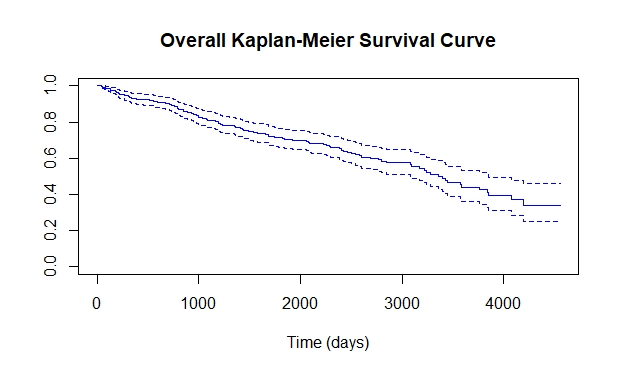
\includegraphics[width=\textwidth]{figs/r_km_overall}
\end{center}
\end{frame}

\begin{frame}[fragile]{Kaplan-Meier estimation example}
	We stratify by treatment group using the formula syntax in \texttt{survfit}:
	\begin{verbatim}
	fit <- survfit(mayo_surv ~ treatment, data = mayo)
	
	plot(fit, 
	col = c("blue","red"),
	lty = 1:2,
	conf.int = FALSE,
	xlab ="Time (days)",
	main = "Stratified Kaplan-Meier Survival Curve")
	
	legend("topright",c("Control","Treatment"),
	    lty = 1:2, col = c("blue","red"))
	\end{verbatim}
\end{frame}

\begin{frame}
\frametitle{Kaplan-Meier estimation example}
	\begin{center}
		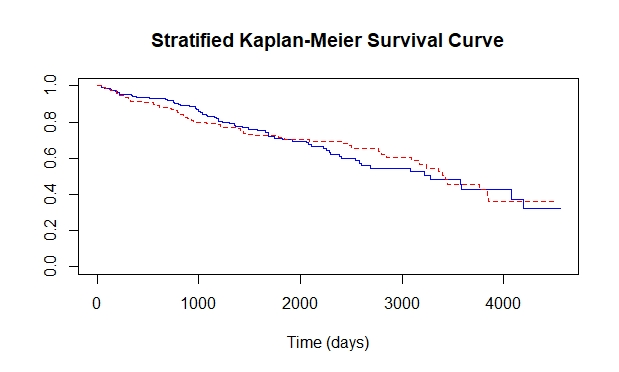
\includegraphics[width=\textwidth]{figs/r_km_strat}
	\end{center}
	What's missing from this plot?   Confidence bands!
\end{frame}

\begin{frame}[fragile]{Kaplan-Meier estimation of survival function}
\vspace{-5 mm}

\footnotesize
\begin{verbatim}
plot(fit, 
col = c("blue","red"),
lty = 1:2,
conf.int = TRUE,
xlab ="Time (days)",
main = "Stratified Kaplan-Meier Survival Curve")

legend("topright",c("Control","Treatment"),
    lty = 1:2, col = c("blue","red"))
\end{verbatim}


	\begin{center}
		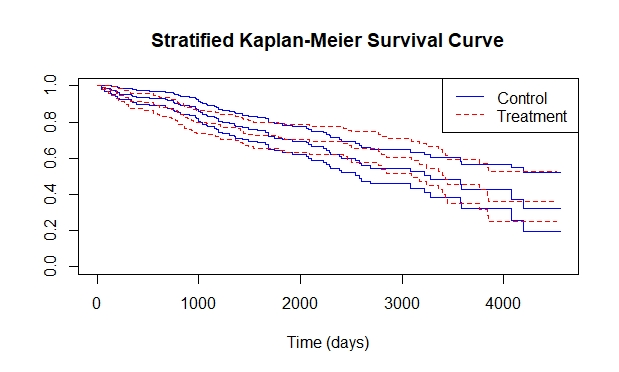
\includegraphics[width=0.8\textwidth]{figs/r_km_strat_ci}
	\end{center}

\end{frame}

\begin{frame}
\frametitle{Estimation of measures of central tendency}

With continuous or binary data, we often used the mean or median to describe the distribution of the variable.
\\ ~\ 

Can we describe the \textbf{central tendency of a distribution} using right-censored data?
\\ ~\ 

Should we (or can we) use the \textbf{mean} or the \textbf{median}?
\begin{itemize}
	
	\medskip
	
\item The mean may be simpler to communicate.

\medskip

\item The median is robust to outliers, while the mean is not.

\medskip

\item Recall that in survival analysis, the mean can be problematic because \textcolor{red}{censoring may render the right tail of the distribution ``unidentifable."}
\end{itemize}
\end{frame}

%\begin{frame}
%\frametitle{Estimation of measures of central tendency}
%
%For this reason, people tend to focus on the \textbf{restricted mean}. We pick some time $\tau$ and integrate the survival curve up to $\tau$: $\mt_\tau := \int_0^\tau S(u) du$; an estimator is given by $\widehat{\mu}_\tau := \int_0^\tau \widehat{S}(u)du$.
%\\ ~\ 
%
%If $\tau$ is not too large, this may be well-defined. 
%\\ ~\ 
%
%The restricted mean is interpreted as the \textcolor{blue}{average survival time, restricted to times less than $\tau$}, or the average of $\min\{T, \tau\}$.
%\\ ~\ 
%
%\textcolor{red}{However, the interpretation of $\mt_\tau$ may not be of interest}, leading people to consider the median instead.
%\end{frame}

\begin{frame}
\frametitle{Estimation of measures of central tendency}
Whenever $S$ is continuous and strictly decreasing, we define the median as the \textbf{timepoint $t_{0.5}$ such that $S(t_{0.5}) = 1/2$}.

\begin{center}
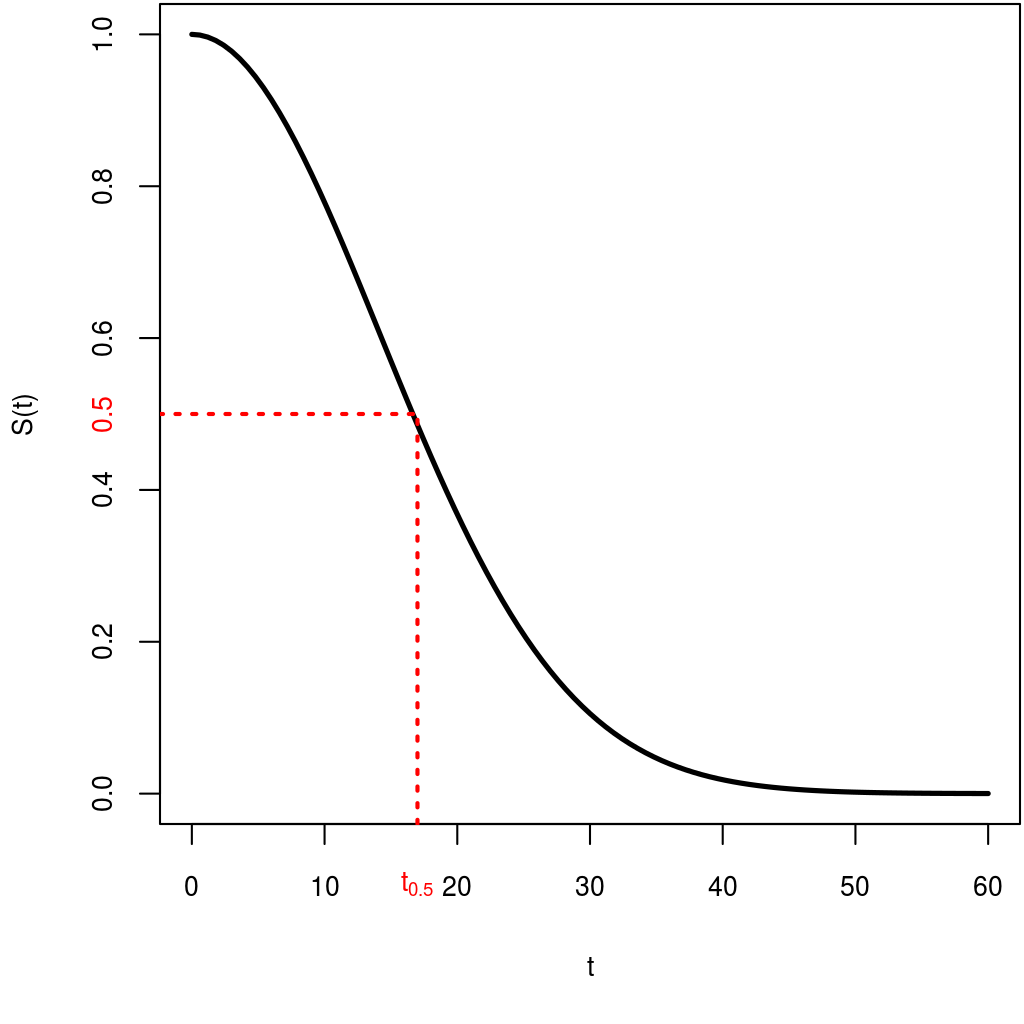
\includegraphics[width=0.7\textheight]{figs/survival_function_median.png}
\end{center}
\end{frame}

\begin{frame}
\frametitle{Estimation of measures of central tendency}
In practice, we will use as estimator of $t_{0.5}$ the median $\hat{t}_{0.5}$ of $\widehat{S}$. But the survival function $\widehat{S}$ is \textbf{not continuous nor strictly decreasing}!

\begin{center}
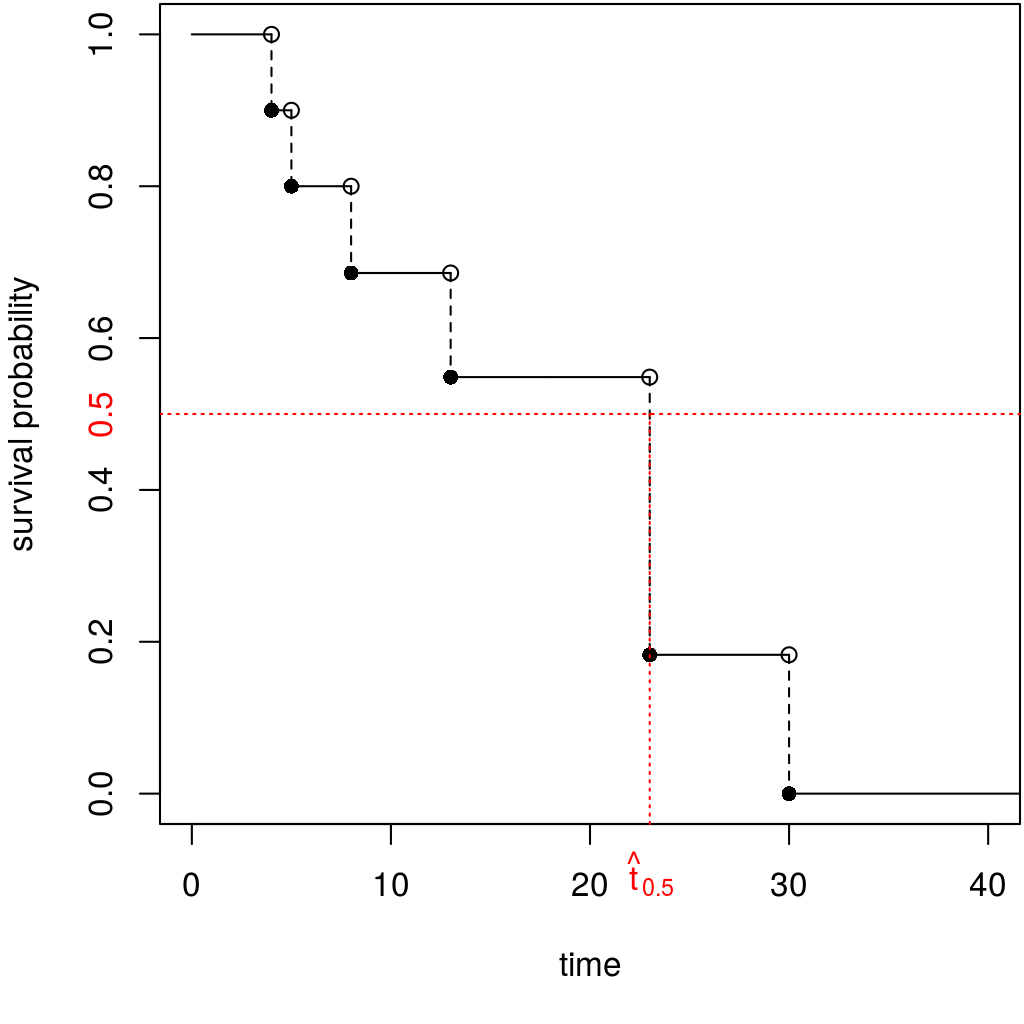
\includegraphics[width=0.6\textheight]{figs/km_small_example_median.png}
\end{center}
Here, $\hat{S}(t)$ jumps from above 0.5 to below 0.5 without hitting it exactly. We'll need to think about what we do here. 
\end{frame}
 

\begin{frame}
\frametitle{Estimation of measures of central tendency}

\vspace{-5 mm}

Some other potential issues: 

\medskip
\begin{enumerate}
\item What if there is no point $\hat{t}_{0.5}$ at which $\widehat{S}$ goes from above to below 0.5?
\begin{center}
	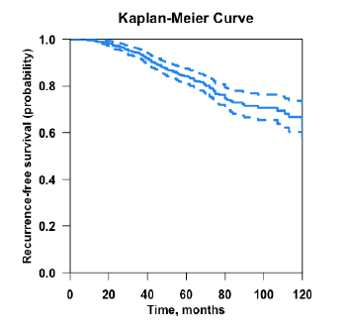
\includegraphics[width=0.6\textheight]{figs/no_median.png}
\end{center}
\item What happens if $\widehat{S}$ equals 0.5 over a whole interval?
\end{enumerate}

\end{frame}


\begin{frame}{Nonparametric esitmation of measures of central tendency}
	To be precise, we'll define the median as the \textcolor{blue}{smallest value $t$ such that $\widehat{S}(t) \leq 0.5$}. This covers us in case the survival curve ``jumps over" 0.5 without hitting it, or is equal to 0.5 over an entire interval of times. 
	\\ ~\ 
	
	In addition, if the estimated survival curve never crosses 0.5, we simply cannot estimate the median survival time. 
	
	\medskip
	
	\textcolor{blue}{If over 50\% of people survive past the end of the study, we have no idea when half of them would get the event.}
	
\end{frame}


\begin{frame}[fragile]{Median of a Kaplan-Meier curve in \texttt{R}} 
	\vspace{-0.5cm}
	
	
	\small
	\begin{verbatim}
	fit <- survfit(mayo_surv ~ 1, data = mayo)
	fit
	
	Call: survfit(formula = mayo_surv ~ 1, data = mayo)
	
	       n events median 0.95LCL 0.95UCL
	[1,] 311    124   3395    3090    3853
	
	summary(fit)$table
	
	records     n.max   n.start    events     rmean se(rmean) 
	311.0000  311.0000  311.0000  124.0000 2981.8864  101.8112 
	median   0.95LCL   0.95UCL 
	3395.0000 3090.0000 3853.0000
	\end{verbatim}
\end{frame}

\begin{frame}[fragile]{Median of a Kaplan-Meier curve in \texttt{R} with multiple groups} 
	\vspace{-0.5cm}
	\small
	\begin{verbatim}
	fit <- survfit(mayo_surv ~ treatment, data = mayo)
	fit
	
	Call: survfit(formula = mayo_surv ~ treatment, data = mayo)
	
	              n events median 0.95LCL 0.95UCL
	treatment=1 157     64   3282    2583      NA
	treatment=2 154     60   3428    3090      NA
	
	summary(fit)$table
	
	            records n.max n.start events    rmean se(rmean) 
	treatment=1     157   157     157     64 2965.551  141.6868   
	treatment=2     154   154     154     60 3002.749  145.7727   
	            median 0.95LCL 0.95UCL
	treatment=1   3282    2583      NA
	treatment=2   3428    3090      NA
	\end{verbatim}
\end{frame}

\begin{frame}
\frametitle{Log-rank test of equal survival between two groups}

It is often of interest to \textcolor{blue}{\textbf{contrast the survival of several groups}}, rather than simply describing the survival time distribution in a single group. 

\medskip
For example, in the Mayo example where we are looking at people being treated for primary biliary cirrhosis:

\medskip
\begin{itemize}
\item Does time to death depend on treatment with d-penicillamine? 
\end{itemize}


\medskip

Commonly, in survival analysis, we \textcolor{blue}{compare the entire survival function between two groups} to answer this question.
\end{frame}

\begin{frame}
\frametitle{Log-rank test of equal survival between two groups}

Comparing the entire survival function is the same as saying that the group-specific time-to-event distributions are identical. Suppose we have groups $Z = 0$ and $Z = 1$, and our outcome is death.
\\ ~\ 

\textbf{Question:} If we want to test for identical time-to-event distributions, what should our null and alternative hypotheses be?   
\\ ~\ 

\textbf{Answer:}
\begin{align*}
\mathbf{\textcolor{blue}{H_0: S_0(t) = S_1(t) \text{\textbf{ for all }} t} \ \text{vs} \ \textcolor{orange}{H_1: S_0(t) \neq S_1(t) \text{\textbf{ for some }}t}}.
\end{align*}   
Note that we need to compare survival across all times! How do we do this? 
\end{frame}

\begin{frame}{Nonparametric testing of equal survivorship between two groups}
At any observed failure time $t$, we can construct a $2 \times 2$ table:

\bigskip

\begin{center}
	\begin{tabular}{c|c|c|c}
		& $Z = 0$ & $Z = 1$ & Overall\\
		\hline
		died & $d_0(t)$ & $d_1(t)$ & $d(t)$ \\
		did not die & $n_0(t) - d_0(t)$ & $n_1(t) - d_1(t)$ & $n(t) - d(t)$\\
		at risk & $n_0(t)$ & $n_1(t)$ & $n(t)$
	\end{tabular}
\end{center}

\medskip

If $H_0$ is true, then we expect that the rows and columns are independent.

\bigskip

 That means we can compute the \textcolor{blue}{expected counts} of deaths and compare to the \textcolor{blue}{observed counts}.
 
 \bigskip
 
 \textit{This should remind you of a Chi-squared test of independence!}
\end{frame}

\begin{frame}
\frametitle{Log-rank test of equal survival between two groups}

\vspace{-7 mm}

\begin{center}
\begin{tabular}{c|c|c|c}
& $Z = 0$ & $Z = 1$ & Overall\\
\hline
died & $d_0(t)$ & $d_1(t)$ & $d(t)$ \\
did not die & $n_0(t) - d_0(t)$ & $n_1(t) - d_1(t)$ & $n(t) - d(t)$\\
at risk & $n_0(t)$ & $n_1(t)$ & $n(t)$
\end{tabular}
\end{center}

\medskip

What do we expect to see in the top-left cell under $H_0$?
\begin{align*}
\textbf{observed count } o(t) &= d_0(t) \\
\textcolor{white}{abc}\\
\textbf{expected count } e(t) &= n(t) \times P(Z = 0) \times P(\text{died}) \text{  (\textcolor{red}{independence!})}\\
\textcolor{white}{abc}\\
&\approx n(t)\times \frac{n_0(t)}{n(t)}\times  \frac{d(t)}{n(t)} = \frac{d(t)n_0(t)}{n(t)}
\end{align*}

\medskip

The expected count is the total sample size times the overall proportion of people in $Z=0$ times the overall proportion of people who died at time $t$.

\end{frame}

\begin{frame}{Log-rank test of equal survival between two groups }
\vspace{-7 mm}

\textcolor{blue}{The difference $o(t) - e(t)$ should be small under $H_0$.} 

\medskip

We can aggregate $o(t) - e(t)$ over \textcolor{orange}{all distinct observed failure times} to get the \textbf{log-rank test statistic}
\begin{align*}
\widehat{T}^2_{LR, n} := \left[\frac{\sum_i \{o(t_i) - e(t_i)\}}{\sqrt{\sum_iv(t_i)}} \right]^2,
\end{align*}

\medskip


\includegraphics[scale = 0.015]{figs/technical} $v(t_i)$, the variance of $o(t_i)-e(t_i)$, is $\frac{n_0(t)n_1(t)d(t)\{n(t)-d(t)\}}{n(t)^2\{n(t) - 1\}}$.

\\ ~\ 

\textcolor{blue}{Under $H_0$, with large sample size the distribution of $\widehat{T}^2_{LR, n}$ is approximately chi-squared with degrees of freedom = the number of groups we are comparing minus 1}

\medskip

P-value for 2 groups is given by $P(\chi^2_1 > x)$!
\\ ~\ 

\textbf{You will never need to do this by hand!}
\end{frame}

\begin{frame}
\frametitle{Log-rank test of equal survival between two groups }
\begin{center}
	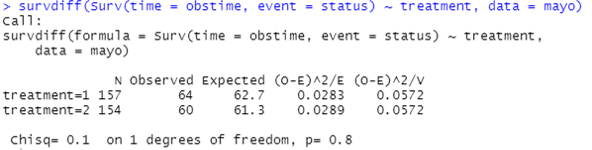
\includegraphics[width=\textwidth]{figs/logrank_code.png}
\end{center}

Using a log-rank test of the null hypothesis of no survival difference at any time between treatment and placebo against the alternative of a survival difference, we fail to reject the null hypothesis at a 0.05 significance level ($p = 0.8$). We do not find statistically significant evidence of a survival difference. 

\end{frame}

%\begin{frame}[fragile]
%\frametitle{Motivation for regression modeling}
%The log-rank test is nice for testing for differences between two groups. 
%\\ ~\ 
%
%If we have a \textcolor{red}{confounder}, we can even adapt the log-rank test by breaking the confounder into discrete categories. But this is pretty limited when we have multiple confounders. 
%\\ ~\
%
%In addition, we'd like to get some \textcolor{blue}{estimate} of association, rather than just a hypothesis test. 
%\\ ~\ 
%
%This is where regression modeling comes in!
%\end{frame}
%
%\begin{frame}{Kaplan-Meier and the log-rank test: summary}
%	\begin{itemize}
%		\item The Kaplan-Meier estimator is a nonparametric (does not make assumptions about the distribution of $T$) method for estimating the survival function while accounting for censoring. We framed it in terms of
%		\begin{itemize}
%			\item Estimating conditional probabilities at each observed time
%			\item Redistribution to the right
%		\end{itemize}
%		\item We can plot Kaplan-Meier curves (with confidence bands) in \texttt{R} using the \texttt{survival} and \texttt{survminer} packages. 
%		\item We can (sometimes) use the Kaplan-Meier curve to estimate the median survival time, which may be of more interest than the mean
%		\item The log-rank test compares the survival functions of two groups
%	\end{itemize}
%\end{frame}
%
%\section{The Cox proportional hazards model}
%\begin{frame}
%\frametitle{Motivation for Cox proportional hazards regression}
%\vspace{-0.8cm}
%With a continuous predictor, we could split the predictor into two subgroups and perform a nonparametric analysis to compare the survivorship between the subgroups.
%\\ ~\ 
%
%For example, we could split \texttt{age} into those under 50 years old, and those over 50 years old, and compare survival:
%
%\begin{center}
%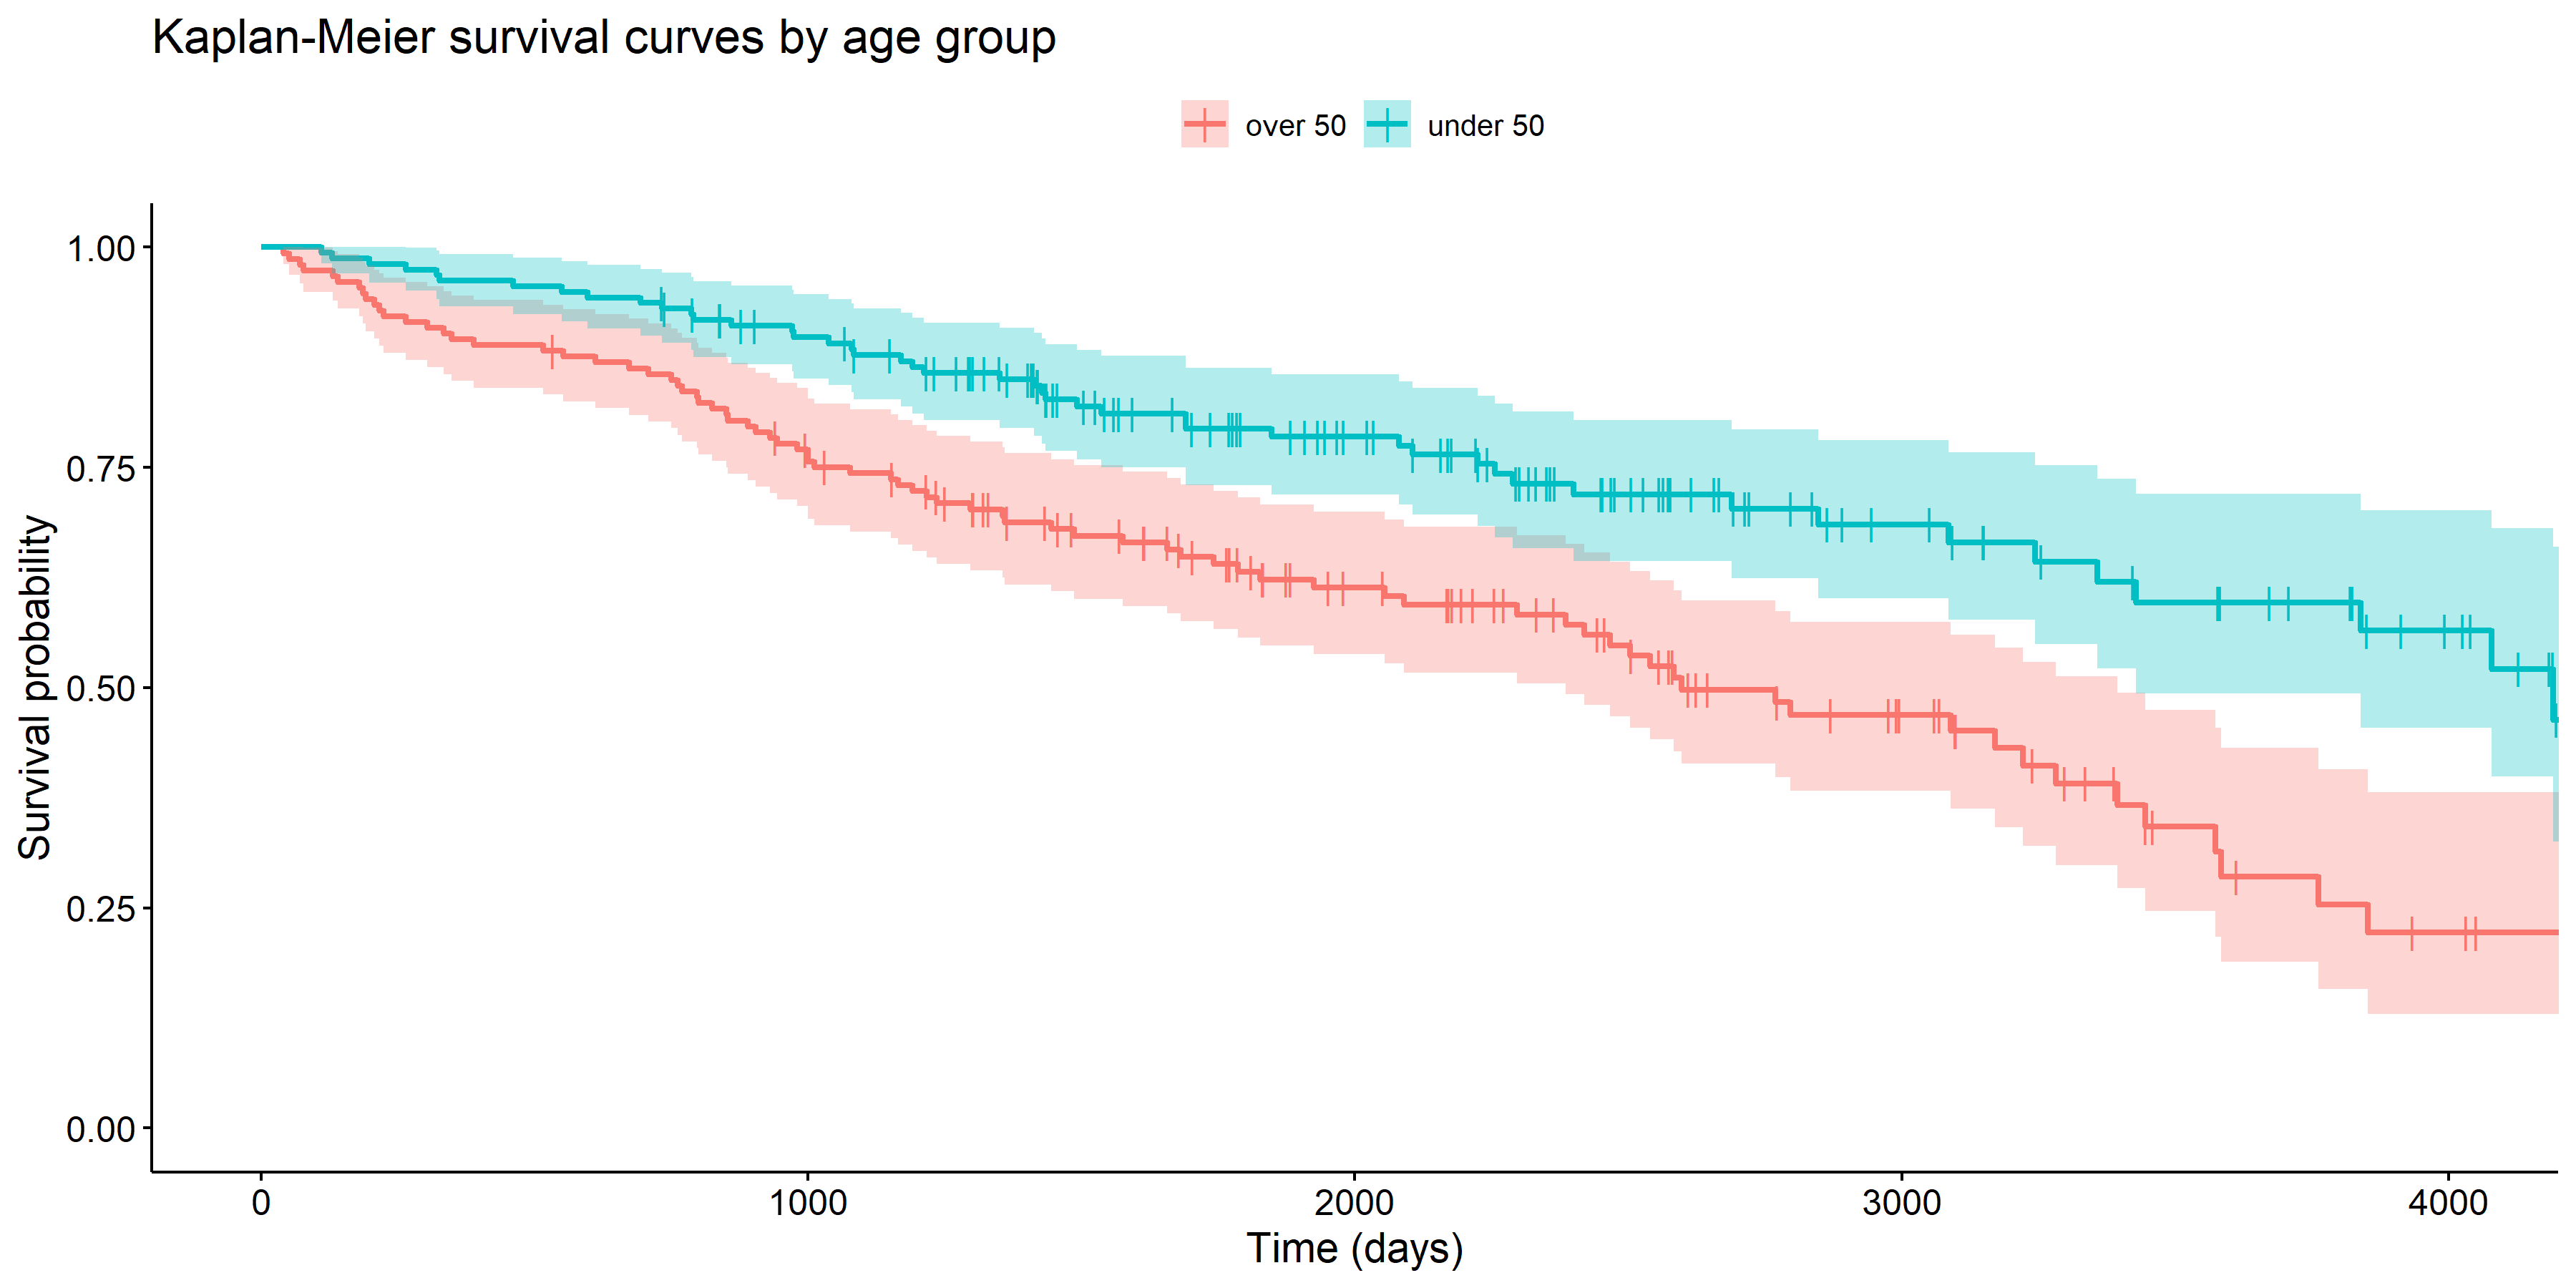
\includegraphics[width = \textwidth]{figs/KM_strat_age.png}
%\end{center}
%\end{frame}
%
%\begin{frame}{Motivation for Cox proportional hazards regression}
%	A log rank test tests the null hypothesis of no survival difference between under and over 50 age groups:
%	\begin{center}
%		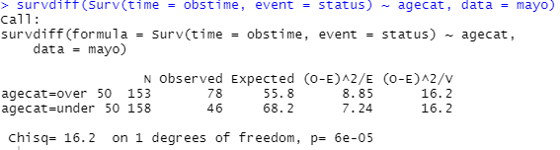
\includegraphics[width = \textwidth]{figs/logrank_agecat.png}
%	\end{center}
%\end{frame}
%
%\begin{frame}
%\frametitle{Motivation for Cox proportional hazards regression}
%
%It appears that the survival probabilities are generally lower (at any point in time) for older versus younger patients. 
%\\ ~\ 
%
%\textbf{Question:} What does this suggest about the \textcolor{blue}{hazards} in the two age groups?  
%
%\textbf{Answer:} Because the younger age group has higher survival probability, we can infer that it also has a lower hazard. 
%\\ ~\ 
%
%If we want to relate the hazard functions between two groups, we might consider a model like
%\begin{align*}
%\textcolor{orange}{h_1(t)} &= c\textcolor{cyan}{h_0(t)},
%\end{align*}
%where $\textcolor{orange}{h_1(t)}$ and $\textcolor{cyan}{h_0(t)}$ are the subgroup-specific hazard functions.
%\end{frame}
%
%\begin{frame}
%\frametitle{The hazard ratio}
%If we only have two groups to compare, we might think about imposing a model on the \textcolor{blue}{ratio of the hazards} of the two groups:
%\begin{align*}
%\frac{\textcolor{orange}{h_1(t)}}{\textcolor{cyan}{h_0(t)}} &= c
%\end{align*}
%This is the simplest example of a \textbf{proportional hazards} model, in which \textit{the hazard functions corresponding to every subgroup considered are proportional to one another.}
%\\ ~\ 
%
%To be a bit more precise, we can re-express this model as
%\begin{align*}
%\frac{\textcolor{orange}{h_1(t)}}{\textcolor{cyan}{h_0(t)}} &= c \text{ for every time } t,
%\end{align*}
%and so, the \textbf{hazard ratio comparing the two subgroups} is \textcolor{red}{constant over time}.
%
%\end{frame}
%
%\begin{frame}
%\frametitle{The hazard ratio}
%The hazard ratio at time $t$ tells us how much more likely it is that an event will happen in subgroup 1 at time $t$ versus in subgroup 0 at time $t$ \textit{given that it has not yet happened in either subgroup.}
%\begin{align*}
%\frac{\textcolor{orange}{h_1(t)}}{\textcolor{cyan}{h_0(t)}} = \frac{\textcolor{orange}{h_1(t)}\Delta t}{\textcolor{cyan}{h_0(t)}\Delta t} \approx \frac{\textcolor{orange}{P(t \leq T < t + \Delta t \mid T \geq t, \text{subgroup }1)}}{\textcolor{cyan}{P(t \leq T < t + \Delta t \mid T \geq t, \text{subgroup }0)}}.
%\end{align*}
%
%\end{frame}
%
%\begin{frame}
%\frametitle{The hazard ratio}
%\begin{align*}
%	\frac{\textcolor{orange}{h_1(t)}}{\textcolor{cyan}{h_0(t)}} &= c \text{ for every time } t,
%\end{align*}
%What does $c < 1$ imply?   A \textbf{decreased hazard} in subgroup 1 relative to subgroup 0. Subgroup 1 is at lower instantaneous risk than subgroup 0 by a factor of $c$.  
%\\ ~\ 
%
%What does $c > 1$ imply?   An \textbf{increased hazard} in subgroup 1 relative to subgroup 0.  Subgroup 1 is at higher instantaneous risk than subgroup 0 by a factor of $c$.
%\end{frame}
%
%\begin{frame}{The hazard ratio}
%	\textbf{Question:} Based on our Kaplan-Meier curves for survival by age group, what can we say about the following hazard ratio?
%	\begin{align*}
%		\frac{h_{\text{over 50}}(t)}{h_{\text{under 50}}(t)}
%	\end{align*}   
%	\textbf{Answer:} Since we saw lower survival over all times for the older versus the younger group (i.e., a larger hazard), we'd expect this hazard ratio to be greater than 1.
%\end{frame}
%
%\begin{frame}
%\frametitle{The hazard ratio}
%Assume that the subgroups are defined so that subgroup 1 has some exposure that we want to show is beneficial (e.g. treatment), while subgroup 0 does not (e.g. placebo):
%
%\begin{enumerate}
%\item If the time-to-event is, e.g., transplant $\rightarrow$ organ rejection or onset of disease $\rightarrow$ death, do we want to observe $c < 1$ or $c > 1$? Why?
%\item If the time-to-event is, e.g., treatment $\rightarrow$ remission, do we want to observe $c < 1$ or $c > 1$? Why?
%\end{enumerate}
%\end{frame}
%
%%\begin{comment}
%\begin{frame}
%\frametitle{The hazard ratio}
%\begin{enumerate}
%\item If the time-to-event is, e.g., transplant $\rightarrow$ organ rejection or onset of disease $\rightarrow$ death, do we want to observe $c < 1$ or $c > 1$? Why?
%\item[] \textcolor{blue}{$c < 1$, because this means that the event tends to occur \textbf{less often} in subgroup 1 than subgroup 0, and events are bad!}
%\item If the time-to-event is, e.g., treatment $\rightarrow$ remission, do we want to observe $c < 1$ or $c > 1$? Why?
%\item[] \textcolor{blue}{$c > 1$, because this means that the event tends to occur \textbf{more often} in subgroup 1 than subgroup 0, and events are good!}
%\end{enumerate}
%\end{frame}
%%\end{comment}
%
%\begin{frame}
%\frametitle{Cox proportional hazards regression}
%In practice, we often have more than two subgroups. In fact, our predictor might be continuous, so defining subgroups isn't straightforward.
%\\ ~\ 
%
%Denoting the hazard function of $T$ given a single predictor of interest $X$ at time $t$ by $h(t \mid X)$, the \textbf{simple proportional hazards model} is:
%\begin{align*}
%\log h(t \mid X) = & \ \log h_0(t) + \beta_1 X,
%\end{align*}
%for each $t$, where $h_0$ is an \textcolor{blue}{unspecified\textsuperscript{*}} hazard function. The model above is the basis of what we call the \textbf{Cox proportional hazards model.}
%\\ ~\ 
%
%How does this relate to the hazard ratio? We'll see!
%\vfill
%\small{\textsuperscript{*}What does this mean? It turns out that to estimate the $\beta_1$ parameter of this model, we don't ever have to deal with $h_0$.}
%\end{frame}
%
%\begin{frame}
%\frametitle{Cox proportional hazards regression}
%Exponentiating both sides of the previous equation, we can model the hazard function as
%\begin{align*}
%h(t \mid X) = & \ h_0(t)e^{\beta_1 X}.
%\end{align*}
%
%Since a survival distribution is completely determined by its hazard function, the distribution of $T$ given $X$ is composed of
%\begin{itemize}
%\item a \textcolor{blue}{coefficient of interest} $\beta_1$: this is how we relate $X$ to the hazard
%\item a \textcolor{blue}{baseline hazard function} $h_0$ (often not of interest): doesn't involve $X$ at all
%\end{itemize}
%\end{frame}
%
%\begin{frame}
%\frametitle{Cox proportional hazards regression: interpretation}
%\vspace{-0.5cm}
%To interpret $\beta_1$, we use our standard approach: 
%\begin{align*}
%h(t \mid X = x + 1) = & \ h_0(t)e^{\beta_1 (x + 1)}\\
%h(t \mid X = x) = & \ h_0(t)e^{\beta_1 x} 
%\end{align*}  \vspace{-0.3cm}
%\begin{align*}
%\textcolor{blue}{\frac{h(t \mid X = x + 1)}{h(t \mid X = x)}} = & \ \frac{h_0(t)e^{\beta_1 (x + 1)}}{h_0(t)e^{\beta_1}} \\
%=& \ \frac{e^{\beta_1x + \beta_1}}{e^{\beta_1 x}} \\
%=& \ \textcolor{blue}{e^{\beta_1 }}
%\end{align*}
%So $e^{\beta_1}$ is the \textbf{hazard ratio} comparing two groups at the same time that differ in $X$ by one unit. 
%\\ ~\ 
%
%We could also say it's the  \textbf{ratio of the instantaneous risk of the event} comparing two groups at the same time that differ in $X$ by one unit.
%\end{frame}
%
%\begin{frame}{Cox proportional hazards regression in \texttt{R}}
%	Estimates of the $\beta$ parameters from proportional hazards regression are (approximately) normally distributed for large sample size, like all of our other regression estimators.
%	\\ ~\ 
%
%	The syntax for Cox proportional hazards regression in \texttt{R} is similar to fitting a linear model or GLM, except
%	\begin{enumerate}
%		\item We use the function \texttt{coxph} in the \texttt{survival} package in \texttt{R}
%		\item Our outcome is a \texttt{Surv} object
%	\end{enumerate}
%	\begin{center}
%		\texttt{coxph(Surv(time, event) $\sim$ X1 + \dots)}
%	\end{center}
%	\begin{itemize}
%	\item This provides naive standard errors. Robust implementations do exist.
%	\item Note that \texttt{coxph}, unlike \texttt{glm}, gives us exponentiated coefficients and confidence intervals! 
%\end{itemize}
%\end{frame}
%
%\begin{frame}{Simple Cox regression: example}
%	Rather than having to arbitrarily binarize age and do a log-rank test, let's instead fit a Cox model: 
%	\begin{center}
%		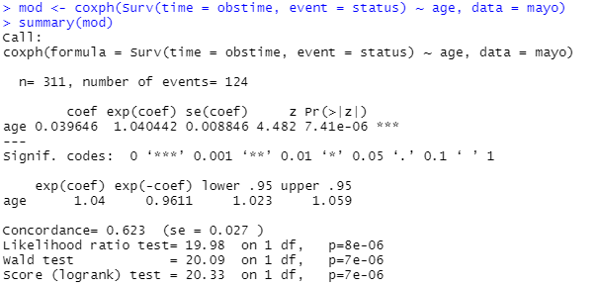
\includegraphics[width = \textwidth]{figs/cox_age.png}
%	\end{center}
%	Use the first p-value in the display (7.41 $\times 10^{-6}$).
%\end{frame}
%
%\begin{frame}{Simple Cox regression: example}
%	We got a hazard ratio of 1.04, with 95\% CI (1.023 - 1.059). In context:
%	\\ ~\ 
%	
%	\textcolor{blue}{We estimate the hazard ratio of death comparing groups one year apart in age is 1.04, with the older group having the higher hazard. The data would not be surprising if the true hazard ratio were between 1.023 and 1.059. We reject the null hypothesis of a hazard ratio of 1 against the alternative that the hazard ratio is not 1 (p $<$ 0.001). There is significant evidence of an association between age and the instantaneous risk of death.}
%\end{frame}
%
%\begin{frame}
%\frametitle{Multiple Cox proportional hazards regression}
%With more than one covariate, we simply extend the model:
%\begin{align*}
%\log \{h(t \mid X_1, \dots, X_p)\} = & \ \log\{h_0(t)\} + \beta_1 X_1 + \dots + \beta_pX_p \\
%h(t \mid X_1, \dots, X_p) = & \ h_0(t)e^{\beta_1X_1 + \dots + \beta_pX_p}.
%\end{align*}
%  
%Now, we interpret the regression parameter $e^{\beta_1}$ as:   \textcolor{blue}{the hazard ratio comparing two groups that differ in $X_1$ by one unit, but are the same with respect to $X_2, \dots, X_p$.}   
%\\ ~\ 
%
%We interpret $e^{\beta_j}$, for $j = 2, \dots, p$, as:  
%\textcolor{blue}{the hazard ratio comparing two groups that differ in $X_j$ by one unit, but are the same with respect to $X_1, \dots, X_{j-1}, X_{j+1}, \dots, X_p$.}   
%\\ ~\
%
%Always keep in mind that hazard = ``instantaneous risk of an event." The term ``hazard ratio" by itself isn't very informative, but it's the more common way to phrase this.
%\end{frame}
%
%\begin{frame}{Cox proportional hazards regression: adjustment variables}
%	Adjusting for \textcolor{red}{potential confounders}, as in all other types of regression we have seen, is necessary if we have observational data and wish to estimate an association between two variables. We do this by adding the potential confounders as covariates in our model.
%	\\ ~\ 
%	
%	When adjusting for \textcolor{green}{precision variables}, as in logistic regression, we don't necessarily reduce our standard errors, so whether to include them or not depends on our scientific question. 
%	\\ ~\ 
%	
%	Finally, as in linear and logistic regression, \textcolor{blue}{effect modification} is assessed using an interaction term that is interpreted as a ratio of ratios.
%\end{frame}
%
%\begin{frame}{Multiple Cox regression: example}
%	\vspace{-0.6cm}
%	Another variable in our dataset is \texttt{stage}, which is an ordinal categorical variable (4 categories) describing the stage of disease at baseline. Here are boxplots of \texttt{age} by \texttt{stage}: 
%	\begin{center}
%		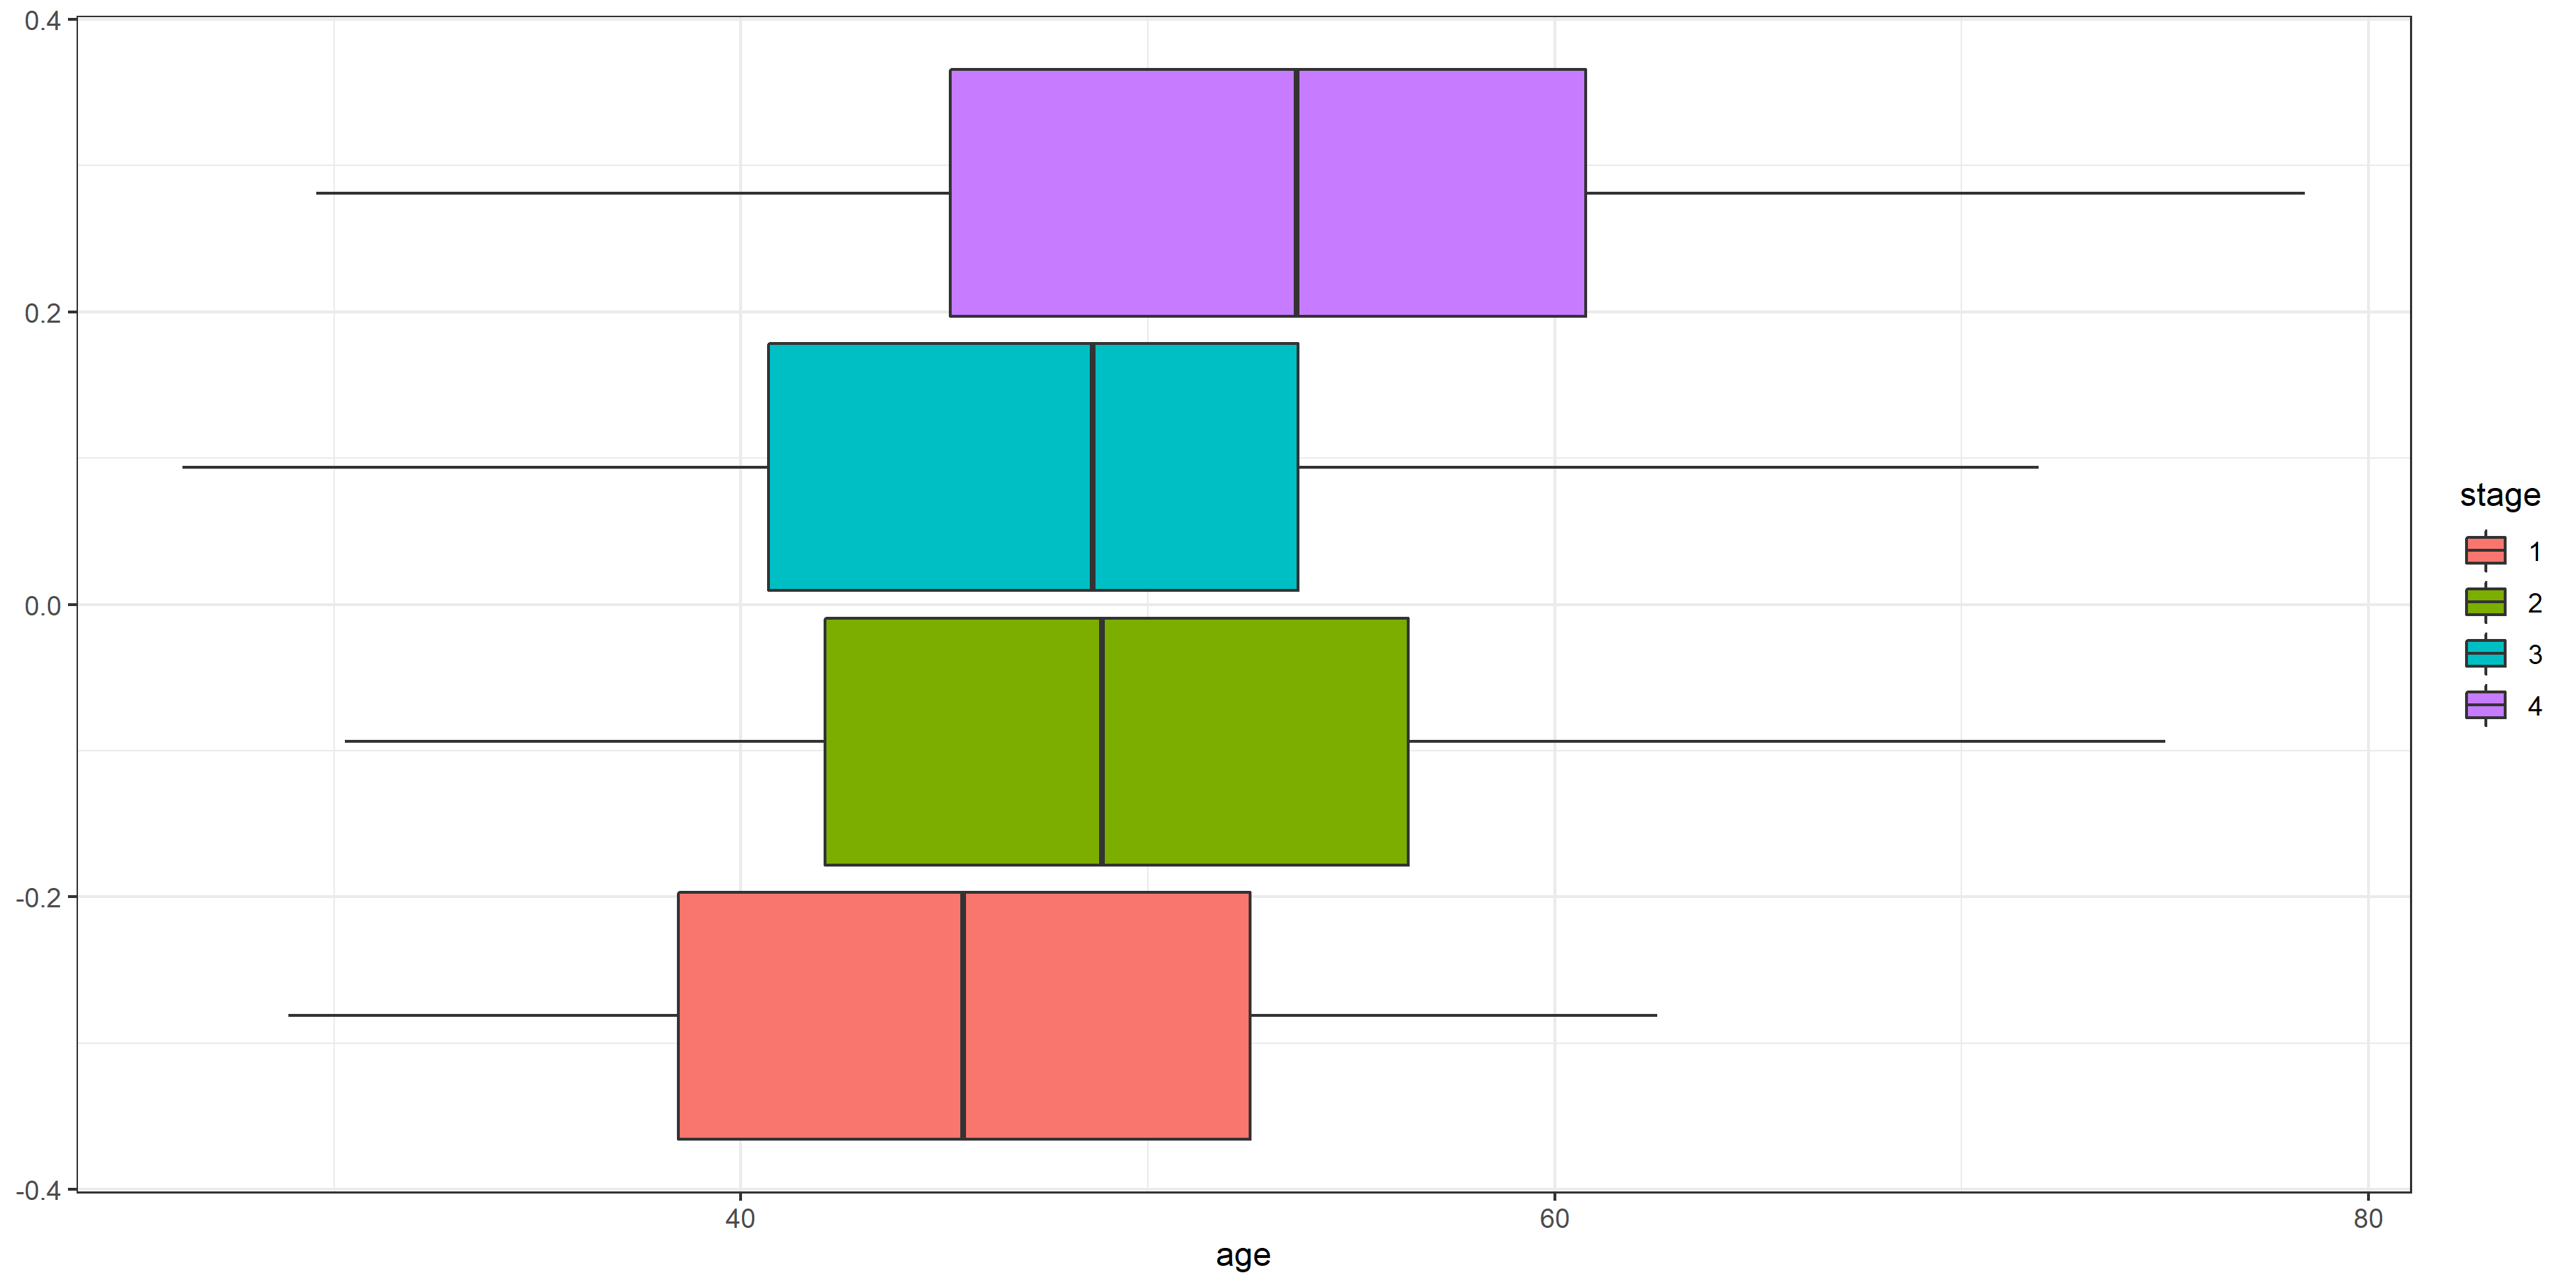
\includegraphics[width = \textwidth]{figs/stage_by_age_box.png}
%	\end{center}
%	If we have reason to believe \texttt{stage} may have a causal effect on survival time, what role does \texttt{stage} play in the association between \texttt{age} and survival?
%\end{frame}
%
%\begin{frame}{Multiple Cox regression: example}
%	So, in order to deal with possible confounding by \texttt{stage}, let's include it in our model:
%		\begin{center}
%		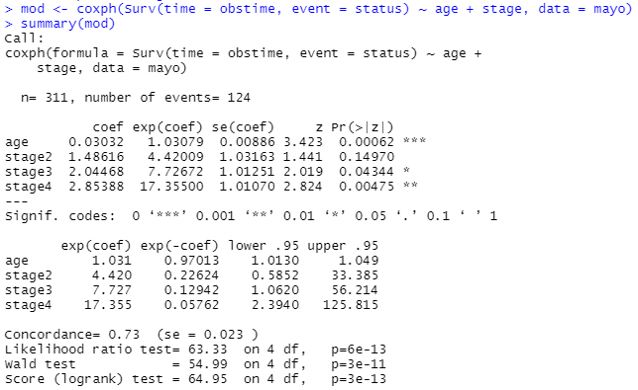
\includegraphics[width = \textwidth]{figs/multiple_cox_regression_code.png}
%	\end{center}
%\end{frame}
%
%\begin{frame}{Multiple Cox regression: example}
%		We got a hazard ratio of 1.03, with 95\% CI (1.013 - 1.049). In context:
%	\\ ~\ 
%	
%		\textcolor{blue}{We estimate the hazard ratio of death comparing groups one year apart in age with the same disease stage is 1.03, with the older group having the higher hazard. The data would not be surprising if the true hazard ratio were between 1.013 and 1.049. We reject the null hypothesis of a hazard ratio of 1 against the alternative that the hazard ratio is not 1 (p $<$ 0.001). There is significant evidence of an association between age and the instantaneous risk of death.}
%\end{frame}
%
%\begin{frame}{Cox proportional hazards regression: effect modification}
%	Suppose we have a predictor of interest $X$ and binary potential effect modifier $Z$. We fit the proportional hazards model
%	\begin{align*}
%		h(t \mid X, Z) = h_0(t)e^{\beta_1X + \beta_2Z + \beta_3XZ}
%	\end{align*}  
%	The hazard ratio comparing groups differing by 1 unit of $X$, for $Z = 0$, is
%	\begin{small}
%	\begin{align*}
%		\frac{h(t \mid X = x+ 1, Z = 0)}{h(t \mid X = x, Z = 0)} = \frac{h_0(t)e^{\beta_1 (x + 1) + 0 + 0}}{h_0(t)e^{\beta_1x + 0 + 0}} = \frac{e^{\beta_1(x + 1)}}{e^{\beta_1 x}} = e^{\beta_1}
%	\end{align*}
%	\end{small}  
%	The hazard ratio comparing groups differing by 1 unit of $X$, for $Z = 1$, is
%	\begin{small}
%	\begin{align*}
%		\frac{h(t \mid X = x+ 1, Z = 1)}{h(t \mid X = x, Z = 1)} = \frac{h_0(t)e^{\beta_1 (x + 1) + \beta_2 + \beta_3(x + 1)}}{h_0(t)e^{\beta_1x + \beta_2 + \beta_3x}} = \frac{e^{(\beta_1 + \beta_3)(x + 1) }}{e^{(\beta_1  + \beta_3)x}} = e^{\beta_1 + \beta_3}
%	\end{align*}
%	\end{small}  
%	The ratio of these two hazard ratios is $e^{\beta_3}$. 
%\end{frame}
%
%\begin{frame}{Cox proportional hazards regression: effect modification example}
%	Does binarized \texttt{sex} (0 = male, 1 = female) modify the association between age and survival?
%	\begin{align*}
%		h(t \mid \texttt{age}, \texttt{sex}) = h_0(t)e^{\beta_1\texttt{age} + \beta_2\texttt{sex} + \beta_3\texttt{sex}\times\texttt{age}}
%	\end{align*}
%			\begin{center}
%		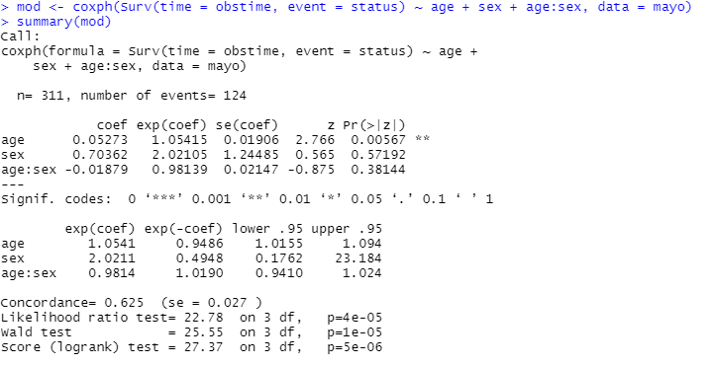
\includegraphics[width = \textwidth]{figs/interaction.png}
%	\end{center} 
%\end{frame}
%
%\begin{frame}{Cox proportional hazards regression: effect modification example}
%	Our estimated (exponentiated) coefficients for \texttt{age} and \texttt{age:sex} were 1.054 and 0.981, respectively.
%	\\ ~\ 
%	
%	Among males (\texttt{sex == 0}), we have a hazard ratio of 1.054, and among females (\texttt{sex == 1}), we have a hazard ratio of $1.054 \times 0.981 = 1.034$.  
%	\\ ~\ 
%	
%	\textcolor{blue}{Among males, we estimate the hazard ratio comparing groups differing by one year in age to be 1.054, with older groups having the higher risk of death. Among females, we estimate the hazard ratio comparing groups differing by one year in age to be 1.034, with older groups having the higher risk of death. This difference in association would not be surprising if the true difference were between 0.941 and 1.024. We do not find significant evidence of effect modification by sex (p $= 0.38$).}
%\end{frame}
%
%\begin{frame}
%\frametitle{Cox proportional hazards regression: assumptions}
%\vspace{-0.5cm}
%Aside from requiring independent censoring, the proportional hazards model makes another strong assumption; specifically, that we have
%\begin{align*}
%\frac{h(t \mid X = x + 1)}{h(t \mid X = x)}=  e^{\beta};
%\end{align*}
%\textit{For each $t$}, the hazard ratio is the same (and is $e^{\beta}$).
%\\ ~\ 
%
%This assumption is violated, for example, if the survival curves cross! 
%\begin{center}
%	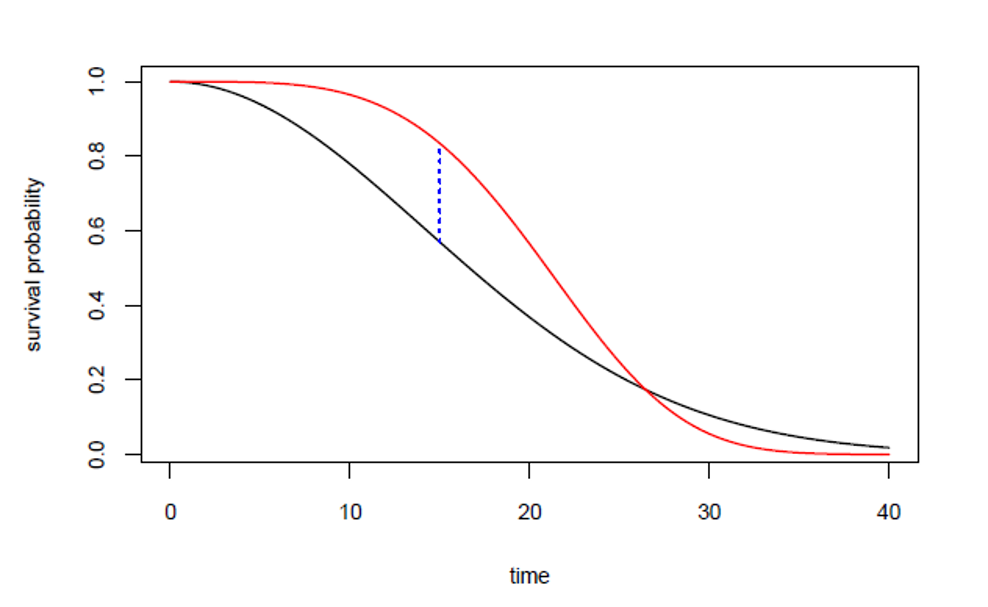
\includegraphics[width = 0.7\textwidth]{figs/crossing_hazards.png}
%\end{center}
%\end{frame}
%
%\begin{frame}{Cox proportional hazards regression: assumptions}
%	If the exposure has a time-varying effect on the outcome, this is unlikely to hold. 
%	\\ ~\ 
%	
%	For example, if you are studying the risk of COVID-19 infection comparing those who have recently been infected to those who have not, you would not expect proportional hazards to hold. 
%	\begin{itemize}
%		\item In the immediate aftermath of an infection, someone is very unlikely to be infected compared to someone who's immunologically naive. 
%		\item Over time, immunity wanes, and reinfection becomes more likely. 
%	\end{itemize}
%
%	There are ways to assess proportional hazards using generalizations of the residual-vs.-fitted plots we saw in Chapter 1, although we won't get into them. For this course, just be aware of how strong this assumption may be.
%\end{frame}
%
%\begin{frame}{The Cox proportional hazards model: summary}
%	\begin{itemize}
%		\item For regression modeling, we focus on comparing the hazards between groups
%		\item The Cox model allows us to estimate the \textcolor{blue}{hazard ratio} comparing groups differing in covariate values
%		\item The Cox model relies on the strong assumption of proportional hazards over all times
%		\item As with other regression methods, we can account for confounding, include precision variables (although they don't work quite the same as in linear regression), and study effect modification
%	\end{itemize}
%\end{frame}
%\section{Summary}
%\begin{frame}
%\frametitle{SECTION 4: SUMMARY}
%Consider the inflammatory biomarkers data; here, normal CRP is $\leq 10$ mg/L, while abnormal CRP is $> 10$ mg/L.
%\begin{center}
%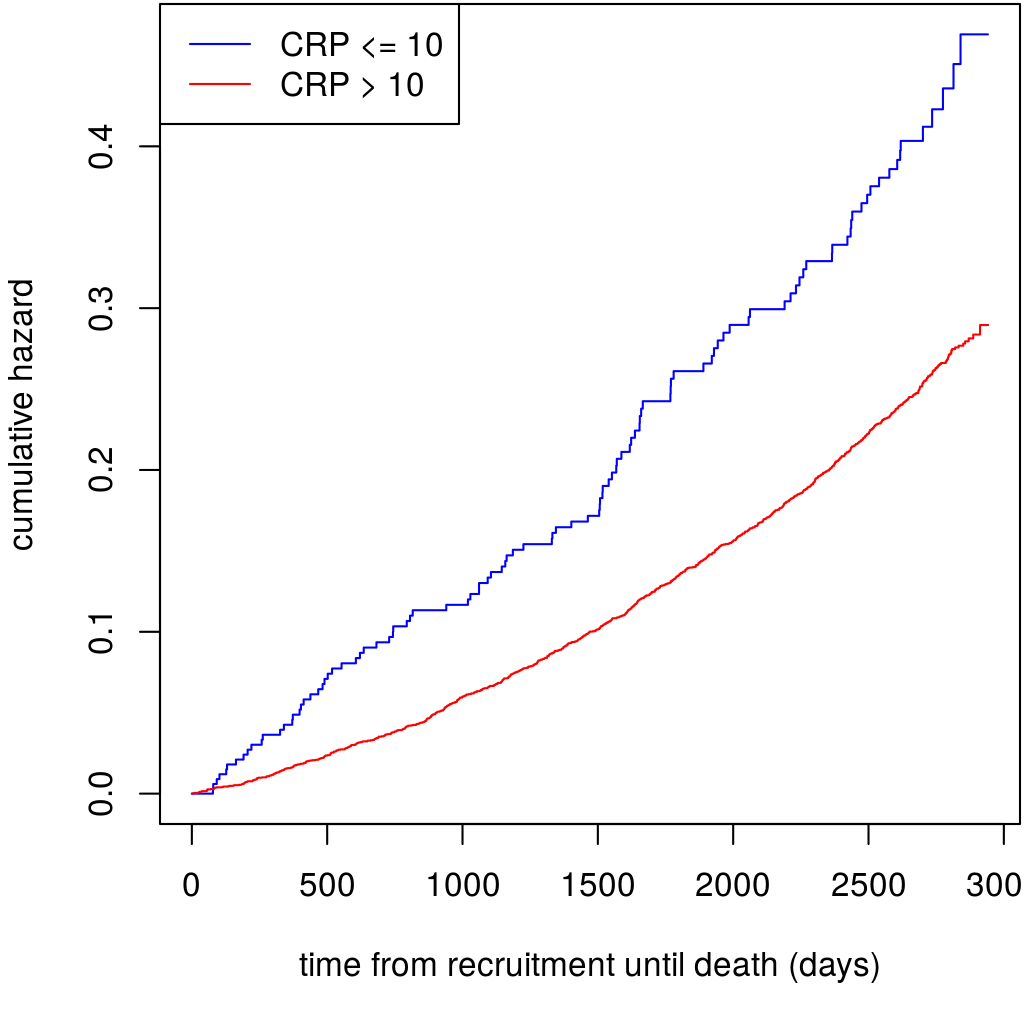
\includegraphics[height = 0.6\textheight]{figs/cum_haz_inflamm_crp.png}
%\end{center} \vspace{-0.6cm}
%First question: is the censoring here informative or uninformative?
%\end{frame}
%
%\begin{frame}
%\frametitle{Survival analysis: CRP}
%\textbf{Scientific question:} Is there \textcolor{orange}{a difference} in \textcolor{blue}{survival} comparing those with normal CRP to those with abnormal CRP?
%
%\textbf{Statistical question:} \vspace{-0.3cm}
%\begin{itemize}
%\item How do we want to quantify the outcome?
%\item[] 
%\begin{itemize}
%\item[]
%\item[]
%\end{itemize}
%\item How will we quantify association?
%\item[] 
%\begin{itemize}
%\item[]
%\item[] 
%\end{itemize}
%\item Are there other variables we need to adjust for?
%\end{itemize}
%\end{frame}
%
%\begin{frame}[noframenumbering]
%\frametitle{Survival analysis: CRP}
%\textbf{Scientific question:} Is there \textcolor{orange}{a difference} in \textcolor{blue}{survival} comparing those with normal CRP to those with abnormal CRP?
%
%\textbf{Statistical question:} \vspace{-0.3cm}
%\begin{itemize}
%\item How do we want to quantify the outcome?
%\item[] \textcolor{blue}{Two options:}
%\begin{itemize}
%\item \textcolor{blue}{Binary variable: survival until prior to first censoring time}
%\item \textcolor{blue}{Time-to-event variable}
%\end{itemize}
%\item How will we quantify association?
%\item[] 
%\begin{itemize}
%\item[]
%\item[] 
%\end{itemize}
%\item Are there other variables we need to adjust for?
%\end{itemize}
%\end{frame}
%
%\begin{frame}[noframenumbering]
%\frametitle{Survival analysis: CRP}
%\textbf{Scientific question:} Is there \textcolor{orange}{a difference} in \textcolor{blue}{survival} comparing those with normal CRP to those with abnormal CRP?
%
%\textbf{Statistical question:} \vspace{-0.3cm}
%\begin{itemize}
%\item How do we want to quantify the outcome?
%\item[] \textcolor{blue}{Two options:}
%\begin{itemize}
%\item \textcolor{blue}{Binary variable: survival until prior to first censoring time}
%\item \textcolor{blue}{Time-to-event variable}
%\end{itemize}
%\item How will we quantify association?
%\item[] \textcolor{orange}{Options (depending on study design):}
%\begin{itemize}
%\item \textcolor{orange}{Binary variable: linear/logistic/Poisson regression}
%\item \textcolor{orange}{Time-to-event variable: difference in survival curves, or hazard ratio}
%\end{itemize}
%\item Are there other variables we need to adjust for?
%\end{itemize}
%\end{frame}
%
%\begin{frame}
%\frametitle{Survival analysis: CRP}
%Survival analysis options:
%\begin{itemize}
%\item Are the \textcolor{blue}{survival curves}  \textcolor{orange}{different}, comparing those with normal CRP to high CRP, with the same \textcolor{orange}{age, diabetes status, sex, BMI, and smoking status?}
%\item Is the \textcolor{orange}{hazard ratio} of \textcolor{blue}{death} different from 1, comparing those with normal CRP to high CRP, with the same \textcolor{orange}{age, diabetes status, sex, BMI, and smoking status}?
%\end{itemize}
%\end{frame}
%
%% KM curves
%\begin{frame}
%\frametitle{Survival analysis: Kaplan-Meier and logrank}
%\hspace*{0.5cm}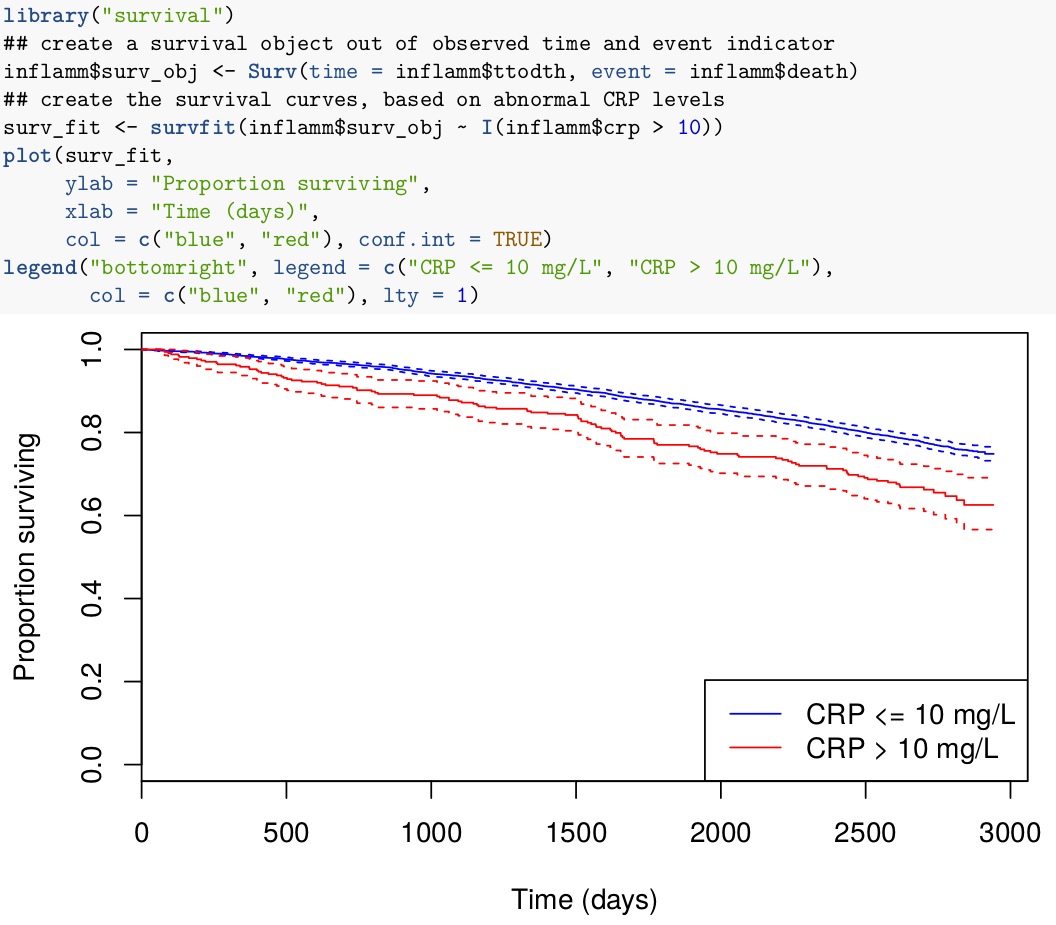
\includegraphics[width=0.9\textwidth]{figs/inflamm_km_crp.png}
%\end{frame}
%
%% unadjusted log rank
%\begin{frame}
%\frametitle{Survival analysis: Kaplan-Meier and logrank}
%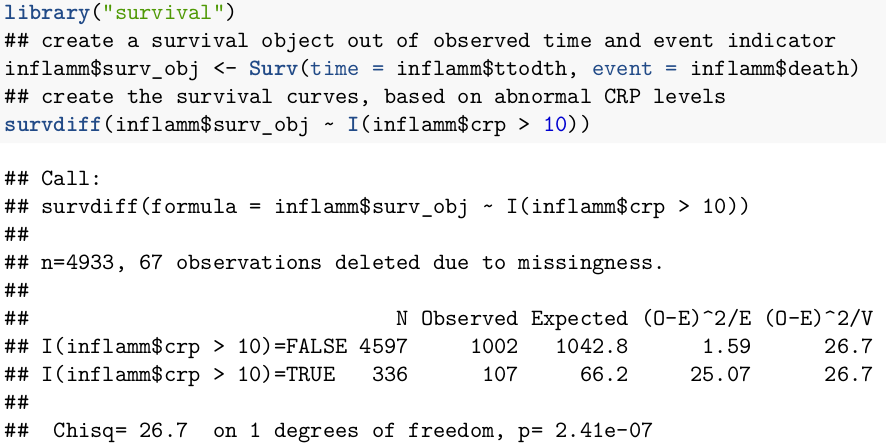
\includegraphics[width = 1\textwidth]{figs/inflamm_logrank_crp.png}
%\end{frame}
%
%% adjusted log rank
%\begin{frame}
%\frametitle{Survival analysis: Kaplan-Meier and logrank}
%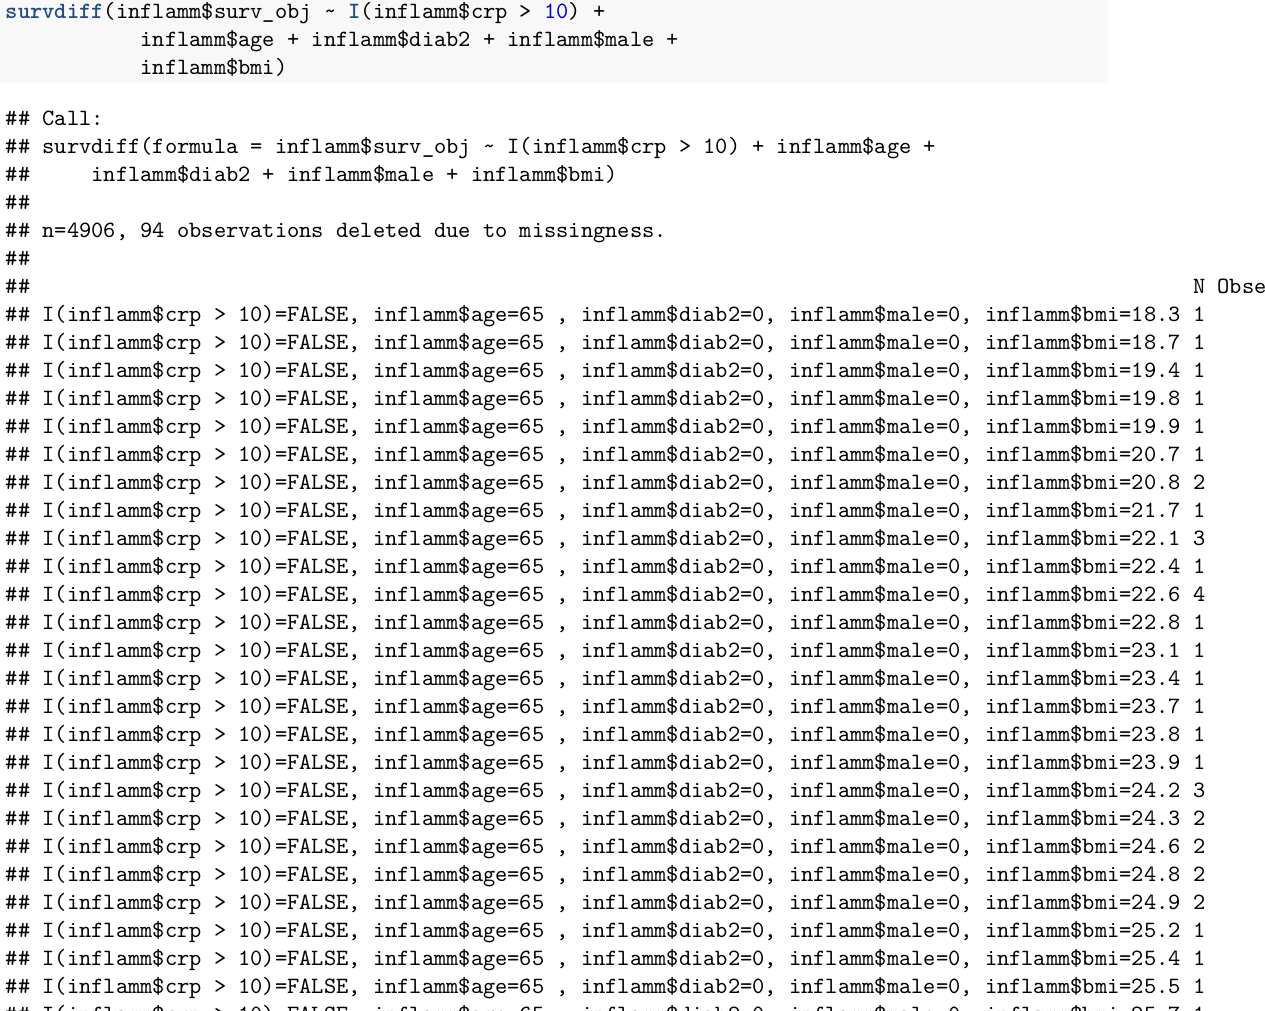
\includegraphics[width = 1\textwidth]{figs/inflamm_logrank_crp_adjust_1.png}
%\end{frame}
%
%\begin{frame}
%\frametitle{Survival analysis: Kaplan-Meier and logrank}
%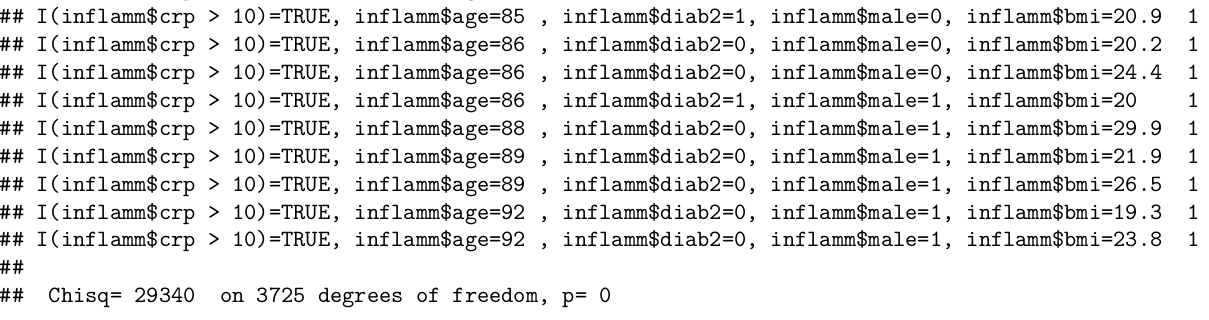
\includegraphics[width = 1\textwidth]{figs/inflamm_logrank_crp_adjust_3.png}
%\end{frame}
%
%\begin{frame}
%\frametitle{Survival analysis: Kaplan-Meier and logrank}
%
%\textcolor{green}{Based on a logrank test}, \textcolor{blue}{these data provide evidence to suggest that the survival function in those with normal CRP is statistically significantly different from the survival function in those with abnormal CRP at the 0.05 level (p $< 0.001$)}. \textcolor{orange}{We conclude that abnormal CRP is associated with decreased survival compared with normal CRP}.
%
%\textcolor{green}{Based on a logrank test}, \textcolor{blue}{these data provide evidence to suggest that the survival function in those with normal CRP is statistically significantly different from the survival function in those with abnormal CRP, among those with the same age, diabetes status, sex, and BMI, at the 0.05 level (p $< 0.001$)}. \textcolor{orange}{We conclude that abnormal CRP is associated with decreased survival compared with normal CRP, adjusting for age, diabetes status, sex, and BMI}.
%\end{frame}
%
%% PH output
%
%\begin{frame}
%\frametitle{Survival analysis: proportional hazards regression}
%Regression model: 
%\begin{align*}
%\log & \{h(t \mid \text{CRP $>$ 10}, \text{Age}, \text{Diabetes}, \text{Male}, \text{BMI}\} =  \log\{h_0(t)\} \\
%&+ \beta_1 (\text{CRP $>$ 10}) + \beta_2 \text{Age} + \beta_3 \text{Diabetes} + \beta_4 \text{Male} + \beta_5 \text{BMI}
%\end{align*}
%\hspace*{0.5cm}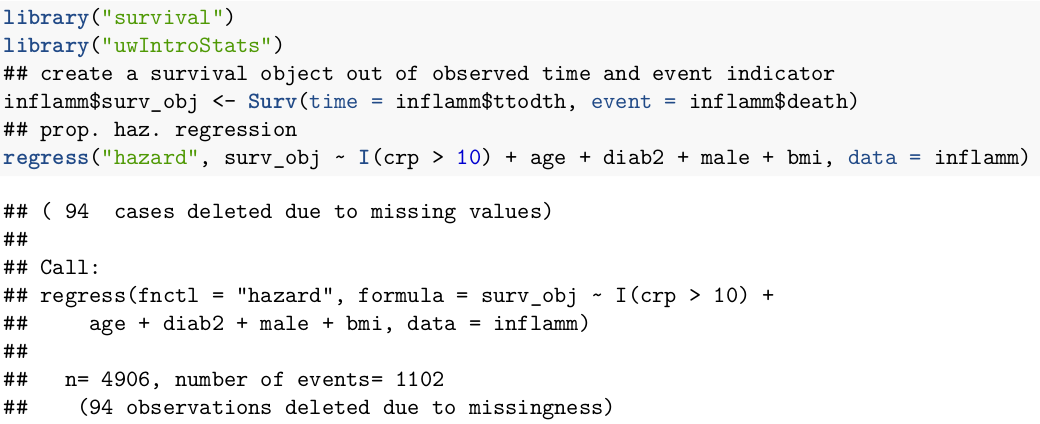
\includegraphics[width=0.9\textwidth]{figs/inflamm_hazard_crp_1.png}
%\end{frame}
%
%\begin{frame}
%\frametitle{Survival analysis: proportional hazards regression}
%\hspace*{0.5cm}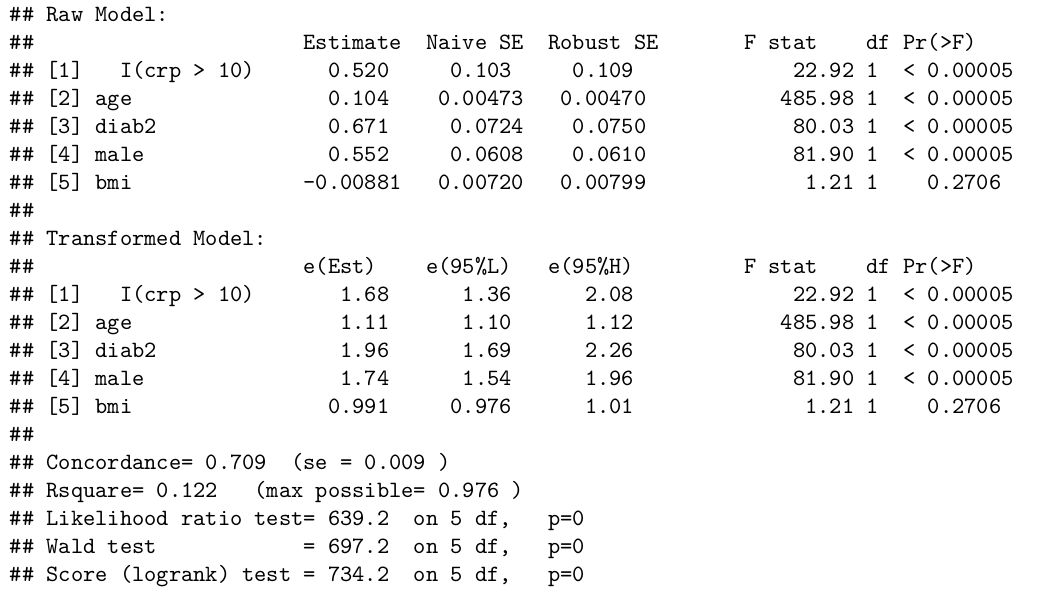
\includegraphics[width=0.9\textwidth]{figs/inflamm_hazard_crp_2.png}
%\end{frame}
%
%% PH reporting results
%\begin{frame}
%\frametitle{Survival analysis: proportional hazards regression}
%Reporting results: 
%\begin{enumerate}
%\item Identify regression coefficient(s) of interest
%\item Report an estimate, and interpret
%\item Report a confidence interval, and interpret
%\item Report a p-value, and interpret
%\item Add a conclusion tying back to the scientific question
%\end{enumerate}
%\end{frame}
%
%\begin{frame}
%\frametitle{Survival analysis: proportional hazards regression}
%\begin{align*}
%\log & \{h(t \mid \text{CRP $>$ 10}, \text{Age}, \text{Diabetes}, \text{Male}, \text{BMI}\} =  \log\{h_0(t)\} \\
%&+ \beta_1 (\text{CRP $>$ 10}) + \beta_2 \text{Age} + \beta_3 \text{Diabetes} + \beta_4 \text{Male} + \beta_5 \text{BMI}
%\end{align*}
%
%Reporting results: 
%\begin{enumerate}
%\item Identify regression coefficient(s) of interest
%\item Report an estimate, and interpret
%\item Report a confidence interval, and interpret
%\item Report a p-value, and interpret
%\item Add a conclusion tying back to the scientific question
%\end{enumerate}
%\end{frame}
%
%\begin{frame}[noframenumbering]
%\frametitle{Survival analysis: proportional hazards regression}
%\begin{align*}
%\log & \{h(t \mid \text{CRP $>$ 10}, \text{Age}, \text{Diabetes}, \text{Male}, \text{BMI}\} =  \log\{h_0(t)\} \\
%&+ \beta_1 (\text{CRP $>$ 10}) + \beta_2 \text{Age} + \beta_3 \text{Diabetes} + \beta_4 \text{Male} + \beta_5 \text{BMI}
%\end{align*}
%
%Reporting results: 
%\begin{enumerate}
%\item Identify regression coefficient(s) of interest: $\textcolor{blue}{e^{\beta_1}}$
%\item Report an estimate, and interpret
%\item Report a confidence interval, and interpret
%\item Report a p-value, and interpret
%\item Add a conclusion tying back to the scientific question
%\end{enumerate}
%\end{frame}
%
%\begin{frame}
%\frametitle{Survival analysis: proportional hazards regression}
%
%\textit{2. Report an estimate, and interpret.}
%
%Based on proportional hazards regression, we estimate that the \textcolor{orange}{ratio of the instantaneous risk of death}, comparing those with abnormal CRP to those with normal CRP but with the same age, diabetes status, sex, and BMI, is \textcolor{orange}{1.68}, where those with abnormal CRP have a higher instantaneous risk of death.  
%
%\textbf{Option 2:} Based on proportional hazards regression, we estimate that the \textcolor{orange}{instantaneous risk of death is 1.68 times higher} among those with abnormal CRP compared to those with normal CRP...  
%
%\textbf{Option 3:} Based on proportional hazards regression, we estimate that the \textcolor{orange}{instantaneous risk of death is 68\% times higher} among those with abnormal CRP compared to those with normal CRP... 
%\end{frame}
%
%\begin{frame}
%\frametitle{Survival analysis: proportional hazards regression}
%
%\textit{3. Report a confidence interval, and interpret.}
%
%Based on a 95\% confidence interval, this estimate would not be judged unusual if the true hazard ratio were between 1.36 and 2.08.
%
%\textit{4. Report a p-value, and interpret.}
%
%These data provide evidence to suggest that this hazard ratio is statistically significantly different from one (p $< 0.001$).
%
%\textit{5. Add a conclusion tying back to the scientific question.}
%
%Based on these results, we have evidence to suggest that the instantaneous risk of death is larger in those with abnormal CRP, after adjusting for age, diabetes status, sex, and BMI.
%\end{frame}

%\begin{frame}
%\frametitle{Survival analysis: assumptions}
%
%Dealing with survival data is complicated, but \textcolor{blue}{we may gain information over simply dichotomizing a time-to-event variable}, and \textcolor{cyan}{sometimes our scientific question does involve the time}.
%
%All of the techniques we have learned rely on the assumption of \textcolor{blue}{uninformative censoring}: those people who are censored are not systematically different from the people in your target population.
%
%This is \textcolor{red}{difficult to assess}, unless you know some additional information about the participants. However, if you are following patients, you may be able to tell based on trends if the patient leaves due to their outcome getting worse.
%
%\end{frame}
%
%\begin{frame}
%\frametitle{Survival analysis: assumptions}
%
%The Kaplan-Meier estimator of the survival function and the logrank test only rely on uninformative censoring -- however, these become difficult to interpret when adjusting for covariates.
%
%The proportional hazards regression model is a convenient alternative, but makes a potentially strong assumption on the hazard ratio between groups defined by the predictor of interest -- namely, that the hazard is proportional at each time $t$.
%
%Despite this limitation, proportional hazards regression is widely used in survival analysis, \textcolor{red}{but the results are often misinterpreted}.
%\end{frame}

\end{document}